\documentclass[a4paper]{cas-sc}

% \usepackage[numbers]{natbib}
\usepackage[authoryear]{natbib}
%\usepackage[authoryear,longnamesfirst]{natbib}

% Author macros
\def\tsc#1{\csdef{#1}{\textsc{\lowercase{#1}}\xspace}}
\tsc{WGM}
\tsc{QE}

\usepackage{amssymb}
\usepackage{amsmath,amsfonts}
\usepackage{caption}
\captionsetup[figure]{name={Fig.},labelsep=period,singlelinecheck=off}
% \usepackage{algorithmic}
\usepackage[linesnumbered,ruled]{algorithm2e}
\usepackage{array}
% \usepackage[caption=false,font=normalsize,labelfont=sf,textfont=sf]{subfig}
\usepackage{textcomp}
\usepackage{stfloats}
\usepackage{url}
\usepackage{verbatim}
\usepackage{graphicx}
% \usepackage{subcaption}
%\usepackage{cite}
%\usepackage{biblatex}  
\usepackage{natbib}
%\usepackage[options]{natbib}
%\addbibresource{ref.bib}
% \hyphenation{op-tical net-works semi-conduc-tor IEEE-Xplore}
% updated with editorial comments 8/9/2021
%\usepackage{hyperref}
\usepackage{subfigure} %By myself
\usepackage{amssymb}
\usepackage{multirow}
\usepackage{mathrsfs}
%\usepackage{mathptmx}
\usepackage{amsthm}
\newtheorem{myDef}{Definition}
\newtheorem{myTheo}{Theorem}
\newtheorem{mypro}{Proposition}
\newtheorem{myex}{Example}
%\usepackage{booktabs}
% \usepackage{algorithmic}
\usepackage{array}
\usepackage{booktabs}
\usepackage{array, caption, threeparttable}
\usepackage[font=small,labelfont=bf]{caption}
\captionsetup[table]{
  labelsep=newline,
  singlelinecheck=false,
}
\usepackage{algpseudocode} 
\usepackage{threeparttable}
\usepackage{hyperref}
\hypersetup{%hypertex=true,
            colorlinks=true,
            linkcolor=blue,
            anchorcolor=blue,
            citecolor=blue}
\usepackage{algpseudocode}
\renewcommand{\algorithmicrequire}{\textbf{Input:}}  % Use Input in the format of Algorithm
\renewcommand{\algorithmicensure}{\textbf{Output:}} % Use Output in the format of Algorithm
\newtheorem{remark}{Remark}   
\renewcommand{\qedsymbol}{}
%reference
\usepackage{hyperref}
\usepackage{threeparttable}


\begin{document}
\let\WriteBookmarks\relax
\def\floatpagepagefraction{1}
\def\textpagefraction{.001}

%------------------------ Title ------------------------

% \title [mode = title]{Subspace Learning Based on Cross-Domain Large Margin Distribution Machine}
\title [mode = title]{Cross-Domain Large Margin Distribution Machine}
\shorttitle{Cross-Domain Large Margin Distribution Machine}

%------------------------ Authors ------------------------
% short author
% \shortauthors{Junlin Chen et~al.}

% %% ---- First Author ----
% \author[1]{Junlin Chen}
% \credit{Methodology, Software, Writing - original draft}
% \affiliation[1]{
%     organization={Schoo of Artificial Intelligence, Southwest University},
%     city={Chongqing},
%     citysep={},
%     postcode={400715}, 
%     country={China}}

% \affiliation[2]{
%     organization={Business school, Jiangsu open University},
%     city={Jiangsu},
%     citysep={},
%     postcode={210036}, 
%     country={China}}

% %% ---- Second Author ----
% \author[1]{Jinrui Guo}
% \credit{Visualization, Data curation}


% %% ---- Third Author ----
% \author[2]{Wenting Hu}
% \credit{Formal analysis, Software}


% %% ---- Fourth Author ----
% \author[1]{Guojun Huang}
% \credit{Writing – review $\&$ editing, Funding acquisition.}


% %% ---- Fifth Author ----
% \author[1]{Libo Zhang}[orcid=0000-0001-5992-0790]
% \credit{Funding acquisition, Validation, Supervision}
% \cormark[1]
% \cortext[cor1]{Corresponding author: Libo Zhang \\
% \qquad \qquad E-mail address: jlchen08@163.com (J. Chen), \\jrguo13@163.com (J. Guo),
% xiaohu\_nanjing@163.com (W. Hu), \\
% aikyoko@163.com (G. Huang),
% lbzhang@swu.edu.cn (L. Zhang)}


%------------------------ Abstract ------------------------
\begin{abstract}
% %由于持续的漂移问题，电子鼻在其应用中受到了严重的限制。支持向量机（SVM）作为一种经典的分类算法，在电子鼻领域中被广泛采用，用于对经过漂移补偿的数据集进行分类。
Due to sensor drift issues, electronic noses (E-noses) are severely limited in their applications. Support vector machine (SVM) aims to reduce classification errors by maximizing the minimum margin, which is widely used to classify drift-compensated datasets in E-noses. 
% % 然而，支持向量机本身并不具备解决电子鼻漂移问题的能力，且其泛化性能有限。
% However, SVM lacks the inherent capacity to directly address drift issues in E-noses, 
% and the generalization performance is also poor, which limits its application in the field of E-noses.
However, the cross-domain learning ability of SVM remains constrained, leading to poor performance in addressing the sensor drift in E-noses.
Moreover, SVM exhibits limitations in terms of generalization, and recent theoretical research has revealed that optimizing the margin distribution result in more superior generalization capabilities than maximizing the minimum margin.
% which has been addressed by the large margin distribution machine (LDM) through incorporating margin distribution.
% 为了解决上述问题，本文提出了一种具有强跨领域学习能力和较高泛化性能的分类器，能够有效应对电子鼻漂移问题。
To address the aforementioned shortcomings, this paper proposes a novel cross-domain large margin distribution machine (CDLDM), which achieves excellent cross-domain learning capabilities and high generalization performance.
% 具体而言，CDLMD旨在通过同时优化源域和目标域之间的投影最大边际分布差异和投影最大分布散射差异，以及边缘分布下的流形一致性来最小化源域和目标域之间的分布差异，从而实现有效的域自适应。
Specifically, CDLDM aims to minimize the distribution discrepancy between source and target domains by simultaneously optimizing the projected maximum marginal distribution discrepancy, projected maximum distribution scattering discrepancy, and the manifold consistency under marginal distribution, thus achieving effective domain adaptation.
% 
% In addition, CDLDM optimizes marginal distribution and achieves better generalization performance than SVM.
In addition, in order to utilize the distribution characteristic information of the samples, the mean and variance optimization terms of the margin distribution are added to the objective function, which further improves the generalization ability of CDLDM.
% 通过在电子鼻数据集上的实验，CDLDM展示了其在跨域学习领域的有效性。
Finally, experiments conducted on the E-noses datasets have demonstrated the significant advantages of CDLDM in the field of E-noses. 
% 综上所述，CDLDM的提出不仅为LDM在跨域学习领域开辟了新的研究方向，也从机器学习角度，为电子鼻漂移问题提供了一种新的、高效的解决方案。
% In summary, CDLDM not only opens new research ***** directions for LDM in the realm of cross-domain learning but also offers a new and efficient solution for sensor drift issues in E-noses.
\end{abstract}
%%Graphical abstract
%\begin{graphicalabstract}
%\includegraphics{grabs}
%\end{graphicalabstract}
%%Research highlights
% \begin{highlights}
% \item TC-IFUPLMC effectively solves the problem of electronic nose drift.
% \item TC-IFUPLMC greatly improves the performance of LDM.
% \item TC-IF strategy solves the inherent problems of  IF strategy.
% \end{highlights}

%------------------------ Highlights ------------------------
% \begin{highlights}
% \item An effective target-domain-free TC-IFUPLMC model is proposed.
% \item TC-IFUPLMC is the first LDM-based model to solve electronic noses drift.
% \item TC-IFUPLMC sensibly enhances the anti-drift performance in electronic noses system.
% \item TC-IFUPLMC has superior disturbance resistance, robustness, and noise resistance.
% \end{highlights}

%------------------------ Keywords ------------------------
\begin{keywords}
Electronic noses\\
Large margin distribution machine\\
Cross domain\\
Sensor drift

\end{keywords}

\maketitle
%% \linenumbers

%% main text
%------------------------ Introduction ------------------------
\section{Introduction}
%电子鼻介绍
Electronic noses (E-noses) consists of a cross sensitive chemical sensor array and a pattern recognition algorithm.
Currently, E-noses are widely employed in diverse domains such as medical diagnostics \citep{DRAGONIERI2009166, DRAGONIERI2007856}, food analysis \citep{DINATALE1997521, PARDO2000397}, and air quality monitoring \citep{DUTTA2003228, JIANG2019108605}. In practical applications, the discriminative capability of E-noses can be compromised by factors such as sensor aging, chemical contamination, and environmental fluctuations, which can induce sensor drift \citep{HOSSEINBABAEI2010641, ZHANG201371, GUNEY201583}. Sensor drift seriously hinders the recognition accuracy of E-noses in practical scenarios \cite{6183455}. As is well known, the drift of E-noses caused by gas sensors can lead to inconsistent distributions of training data and test data, thus causing cross-domain problems \cite{6963383}.
In order to facilitate comprehension, we offer a succinct explanation of cross-domain issues. 
% Suppose ${{X}_{1}},\ldots ,{{X}_{n}}$ represents the data collected by the sensor, where $X$ is called the source domain (no drift), and $n$ batches are arranged in time intervals. ${{p}_{1}}$ represents the distribution of the source domain data.
Let ${{X}_{1}},\ldots ,{{X}_{n}}$ represent the source domain, and the distribution of the source domain is represented by ${{p}_{1}}$.
${{Y}_{1}},\ldots ,{{Y}_{n}}$ represent the target domain and ${{p}_{2}}$ represents its distribution. 
% The drift issue refers to the fact that when ${{p}_{1}} \ne {{p}_{2}}$ ( the distribution of the two is inconsistent), the E-noses classifier used for labeling training with source domain data has significantly lower test performance on the target domain. 
The drift issue refers to the fact that the distributions of two domains are inconsistent, i.e., ${{p}_{1}} \ne {{p}_{2}}$. In this scenario, an E-nose classifier trained on data from the source domain often exhibits significantly reduced performance when tested on data from the target domain \cite{di2012drift}.
As the aging of sensor increases, the discrepancy between the distributions of ${{X}_{1}},\ldots,{{X}_{n}}$ and ${{Y}_{1}},\ldots,{{Y}_{n}}$ grows more pronounced, leading to a degradation in the classifier's generalization capabilities.


%灵感来源---跨域SVM
%Traditional LDM assumes that the data distribution between training and testing data is similar. Consequently, it faces limitations in solving cross-domain problems and demands structural adaptations. At present, some domain adaptation methods based on SVM have been proposed to solve cross-domain problems. Long et al.[] proposed a new transfer learning framework called Adaptive Regularization Based Transfer Learning (ARTL). ARTL learns an adaptive classifier by simultaneously optimizing the structural risk function, joint distribution matching between domains, and manifold consistency under marginal distribution. Under the ARTL framework, Long et al. proposed ARSVM and derived corresponding solutions using the Representer theorem in reproducing kernel Hilbert spaces. Tao et al.[] constructed the Generalized Projection Maximum Distribution Difference (GPMDD) metric based on the reproducing kernel Hilbert Space (RKHS) domain distribution by simultaneously considering the mean and scattering differences of the maximum projection distribution between the source and target domains. Based on the principles of structural risk and GPMDD minimization, Tao et al. proposed a new domain adaptive kernel support vector machine (DAKSVM).
% In addressing the E-noses drift issues, a common approach is initially compensating for drift data to make the distribution of source and target domain data consistent followed by the application of support vector machine (SVM) for classification \citep{YAN2022107664, ZHANG2017407, GUO2022118237}.
To address the issue of sensor drift in E-noses, a prevalent method is compensating for the drift data to ensure the alignment of the source and target domain distributions. Subsequently, a support vector machine (SVM) classifier is employed to classify \citep{YAN2022107664, ZHANG2017407, GUO2022118237}.
While this strategy often yields favorable outcomes, it is also with potential drawbacks. SVM operates under the assumption of identical data distribution between the training and testing datasets, i.e., ${{p}_{1}} = {{p}_{2}}$. Consequently, it faces limitations in solving cross-domain problems. Despite compensating for data drift, SVM neglects distribution discrepancy between various domains during training, potentially hindering optimal performance in certain scenarios. 

At present, some domain adaptation methods based on SVM have been proposed to solve cross-domain problems. Long et al. \citep{ARTL} proposed a new transfer learning framework called adaptive regularization based transfer learning (ARTL). ARTL learns an adaptive classifier by simultaneously optimizing the structural risk function, joint distribution matching between domains, and manifold consistency under marginal distribution. Under the ARTL framework, Long et al. proposed ARSVM \citep{ARSVM} and derived corresponding solutions using the representer theorem in reproducing kernel Hilbert spaces. 
Tao et al. \citep{TAO20123962} have developed the generalized projection maximum distribution difference (GPMDD) measure, which is grounded in the reproducing kernel hilbert space (RKHS) domain distribution. This measure takes into account both the mean and scattering differences of the maximum projection distributions, thereby providing a nuanced assessment of the distributional variations.
Based on the principles of structural risk and GPMDD minimization, Tao et al. \citep{TAO20123962} proposed a new domain adaptive kernel support vector machine (DAKSVM). The above models have achieved good cross-domain processing performance to a certain extent, but they only adopt some cross-domain processing methods, ignoring some important methods. In addition, these models are all improved under the SVM model and still lack consideration for marginal distribution.

SVM aims to maximize the minimum margin between the support vector and the classification hyperplane\citep{Reyzin,zhang2018optimal,9225727}. However, according to the marginal theory, the marginal distribution plays a more crucial role than the minimum margin in enhancing the model's generalization capability \citep{GAO20131,wang2011refined}.
% Based on marginal theory, Zhang et al.\cite{LDM} proposed the large margin distribution machine (LDM), which achieves  best generalization performance by optimizing the marginal distribution. 
Inspired by these results, Zhang et al. \cite{LDM} first focused on the influence of marginal distribution on SVM and proposed the large margin distribution machine (LDM). By incorporating two second-order statistical measures, the construction of the classification hyperplane is affected by all sample points rather than being confined to the support vectors alone \citep{stephan}. Hence, this comprehensive consideration of data points is posited to yield superior generalization performance in comparison to the traditional SVM methodology.
% In the context of LDM, the classification hyperplane is influenced by the collective contribution of all sample points, rather than being solely determined by the support vectors. This comprehensive consideration of data points is posited to yield superior generalization performance in comparison to the traditional SVM methodology \citep{stephan}. 
Despite its widespread application, LDM has predominantly been employed in addressing single-domain problems and exhibits limited efficacy in resolving cross-domain challenges.

%CDLDM
%Taking inspiration from previous work, we consider the global distribution differences of data and extend LDM to cross-omain learning domains. %To this end, we propose an novel Cross-Domain Large Margin Distribution Machine (CDLDM) with excellent cross-domain learning capabilities. Specifically, our research aims to achieve effective domain adaptation by minimizing the distributional discrepancy between the training data from the source domain and the test data from the target domain. To accomplish this objective, we simultaneously optimize the projection maximum marginal distribution discrepancy and the projection maximum distribution scatter discrepancy between the source and target domains, along with the manifold consistency under marginal distribution to learn an adaptive classifier and use the Representer theorem to derive the corresponding solution in the Reproducing Kernel Hilbert Space (RKHS). Finally, we conduct a series of comprehensive experiments on different sensor drift data sets to empirically verify the cross-domain learning ability of CDLDM. In summary, the main contributions of this work are as follows:
Inspired by previous researches, we extend LDM to the cross-domain learning domain by considering the global distribution differences of data and propose a novel cross-domain large margin distribution machine (CDLDM) with excellent cross-domain learning capabilities and high generalization performance. 
% Specifically, CDLDM aims to achieve effective domain adaptation by minimizing the distribution difference between the training data of the source domain and the test data of the target domain. To achieve this goal, we simultaneously optimize the projected maximum marginal distribution difference and the projected maximum distribution dispersion difference between the source and target domains, as well as the manifold consistency under the marginal distribution to learn an adaptive classifier, and use a representation The theorem derives the corresponding classifier. Solution in Reproducing Kernel Hilbert Space (RKHS). 
Specifically, CDLDM aims to minimize the distribution difference between the source domain and the target domain by simultaneously optimizing the projected maximum marginal distribution difference, the projected maximum distribution dispersion difference, and the manifold consistency under the marginal distribution, thus achieving cross-domain learning. In addition, CDLDM also optimizes marginal distribution and demonstrates superior generalization performance than SVM.
Compared with the previous method of compensating for drift data before applying SVM classification, CDLDM extends SVM to cross-domain learning domains, enabling it to directly classify drift data and possessing excellent generalization ability.
We conduct a sequence of comprehensive experiments on different sensor drift datasets to empirically verify the cross-domain learning capability of CDLDM. The principal contributions of this paper are synthesized in the following key points:

\begin{itemize}
   \item [$\bullet$]To the best of our knowledge, this paper extends LDM to the field of cross-domain learning for the first time, greatly enhancing the cross-domain learning capabilities of LDM.
   
    \item [$\bullet$] From the perspective of machine learning, we provide a new and efficient solution to the sensor drift problem. The proposed CDLDM is a domain adaptive classifier that has cross-domain capabilities and effectively solves the problem of distribution inconsistency caused by drift.
    
    \item [$\bullet$] Based on a series of comprehensive experiments on different E-noses datasets, consistent findings highlight the excellent cross-domain learning capabilities exhibited by CDLDM. Notably, our proposed model outperforms some classical models.
\end{itemize} 

% The subsequent sections of this paper are organized as follows. Section \ref{rel} provides a brief description of the drift compensation for gas sensors, as well as introduces LDM. In Section \ref{novel}, a novel CDLDM classification model and its solution are presented. In Section \ref{Experiments}, a comprehensive set of experiments is conducted using various sensor drift datasets to showcase the superior anti-drift performance of our model. Finally, Section \ref{Conclu} draws conclusions and provides future research directions.
The structure of the remaining sections of this manuscript is outlined below.
Section \ref{rel} delineates a succinct overview of the literature on drift compensation techniques for gas sensor, while concurrently introducing the LDM. Section \ref{novel} proposes the CDLDM, along with its algorithmic solution. In Section \ref{Experiments}, an extensive experimental protocol is elaborated, wherein a diverse array of sensor drift datasets is utilized to demonstrate the enhanced robustness against drift of the proposed model. Conclusively, Section \ref{Conclu} synthesizes the findings of this study.



%------------------------ Related work ------------------------

\section{ Related Work}\label{rel}
In this section, we briefly introduce some background knowledge of sensor drift compensation and LDM.

\subsection{Drift Compensation for Gas Sensors}\label{II-A}

% %电子鼻介绍
% E-noses are a kind of cross-sensitive gas sensor arrays with intelligent signal processing and pattern recognition units. At present, E-noses are widely used in various fields, such as air quality monitoring, food analysis, and medical diagnosis. \textcolor{blue} {Within practical operational domains, the discernment capabilities of electronic noses (E-noses) may be compromised by sensor drift, stemming from factors like sensor aging, chemical poisoning, and fluctuations in ambient environmental variables such as humidity and temperature. This phenomenon imposes constraints on the reliability and accuracy of E-noses in applied contexts.}%修改了语言，同时将长难句变为两个整句。


%漂移补偿方法---分量校正
% In current research, addressing the drift problem is primarily categorized into three approaches: the first is drift component correction methods; the second is adaptive methods; and the third is machine learning techniques. The objective of drift component correction strategies is to identify and eliminate drift components inherent in original signals prior to classifier training. This methodology relies predominantly on reference samples or component removal techniques. In the case of the former, Haugen et al. [] introduced a mathematical drift compensation algorithm hinging on correction samples. However, this method imposes stringent demands on calibration samples, necessitating a high correlation with the target sample and comparable sensor responses and drift behaviors. For the latter category, a straightforward drift component correction  method named CC-PCA [] employs principal component analysis to mitigate sensor drift. This technique identifies the drift direction and eliminates the component aligned with this drift direction from the measured values. Another approach, orthogonal signal correction (OSC) [], proposed by Padilla et al., identifies components orthogonal to the signal as drift and directly removes them. However, it is worth noting that these methods might run counter to the fundamental nature of drift, as they assume drift to be additive noise and attempt additive correction of the drift components.

In contemporary research, the resolution of the drift issues is principally stratified into three approaches: 1. drift component correction methods; 2. adaptive methods; 3. machine learning techniques. 
Drift component correction strategies aim to identify and eliminate inherent drift components in original signals before classifier training. This methodology relies on reference samples or component removal techniques. 
Haugen et al. \cite{haugen2000calibration} introduced an algorithmic framework for mathematical drift compensation, which is predicated on the utilization of correction samples to achieve enhanced calibration accuracy, yet it imposes stringent demands on calibration samples, requiring a high correlation with the target sample and comparable sensor responses and drift behaviors. Another approach, the orthogonal signal correction (OSC) model proposed by Padilla et al.\citep{padilla2010drift} identifies and removes drift by targeting components orthogonal to the signal.

% orthogonal signal correction (OSC) by Padilla et al. \citep{padilla2010drift}, identifies components orthogonal to the signal as drift and directly removes them. 
% However, it's crucial to note that these methods may contradict the fundamental nature of drift, assuming it as additive noise and attempting additive correction of the drift components.

%漂移补偿方法---域自适应
%整体润色，删除不必要的
%\textcolor{blue}{Domain adaptation approaches are broadly categorized into feature adaptation and classifier adaptation methods. Classifier adaptation primarily aims to facilitate effective knowledge transfer across diverse domains, as evidenced by Vergara et al.'s endeavors in addressing prolonged gas sensor drift through the construction of an ensemble comprising multiple weighted classifiers.In contrast, adaptive feature transfer methods concentrate on mitigating probability distribution differences among diverse domains. Zhang et al. introduced a domain-regularized component analysis (DRCA) model for this purpose, identifying a latent subspace to minimize distributional differences between two domains. Building upon this foundation, Yi et al. augmented DRCA by incorporating label information from the source data, introducing a more efficient variant recognized as discriminative DRCA (D-DRCA).}
Adaptive compensation is a method to address drift by dynamically adjusting coefficients in pattern recognition algorithms to align with current sensor outputs. This proves effective for tackling time-varying drift challenges. Proposed strategies, such as Adaptive Resonance Theory \citep{DISTANTE2000248} and Self-Organizing Maps (SOM) \citep{zuppa2004drift}, exhibit notable effectiveness in drift suppression. However, their success relies heavily on accurate model classification, with misclassifications potentially compromising the model's ability to track patterns accurately. 
% Holmberg et al. \citep{HOLMBERG1997185} introduced an implicit dynamic variation model to suppress common-mode drift in sensor outputs.
Inspired by Martinelli et al.'s \citep{MARTINELLI20131017} artificial immune system, an adaptive classifier was integrated to mitigate drift impacts. Despite these advancements, their reliance on precise model classification and the need for frequent recalibration in practical scenarios pose inherent limitations, resulting in increased implementation costs and system complexity. 
% The pursuit of long-term stability and robustness in electronic nose systems remains an ongoing challenge. Future research may contemplate integrating diverse compensation methodologies to fortify the system's resilience against drift and simultaneously reduce complexities associated with system maintenance.

% **********更换（Sensor Drift Compensation of E-nose Systems with Discriminative Domain Reconstruction Based on an Extreme Learning Machine）

%漂移补偿方法---机器学习
%整体润色
Machine learning methodologies are engineered for mitigating the impact of data drift or shift, with an emphasis on minimizing these effects without explicitly characterizing the nature of the drift or shift. 
% These strategies can be broadly categorized into two classes: decision-based  and feature-based.
Machine learning methodologies are classified into two main classes: decision-based and feature-based. 
Decision-based strategies aim to directly enhance the classifier's adaptability to drift \citep{8846675, VERGARA2012320}. 
% In contrast, feature-based strategies involve the initial identification of an intrinsic feature subspace where the original data and drifted data closely align. 
% In contrast, feature-based strategies are compensating for the drift data in intrinsic feature subspace to ensure the alignment of the source and target domain distributions. 
In contrast, feature-based strategies first compensate for drift data in the feature subspace to ensure the alignment of the source and target domain distributions.
Subsequently, traditional machine learning models are applied in this subspace for classification \citep{YAN2022107664, ZHANG2017407, GUO2022118237}.

LDM promotes the generalization ability of traditional SVM by optimizing the margin distribution, diverging from the exclusive focus on minimizing the maximum margin. Despite its widespread application, LDM has predominantly been employed in addressing single-domain problems and exhibits limited efficacy in resolving cross-domain challenges. To address drift issues in E-noses data more effectively, we extend LDM to the field of cross-domain learning and proposed a novel CDLDM. In contrast to previous methodologies, which initially seek to align the distributions of original and drifted data in a subspace before applying machine learning techniques for classification, our approach simultaneously minimizes distribution differences between domains and classifies. This novel approach aims to offer a more efficient solution for mitigating drift-related challenges in E-noses systems.





% \subsection{Subspace Learning}\label{II-B}

% The basic concept of subspace learning is to transform the observed data from the perceived high-dimensional space to the low-dimensional subspace, where the key knowledge and specific characteristics of the data are well preserved and redundant noise information is removed, and the basic methods are principal component analysis (PCA) and linear discriminant analysis (LDA). However, these traditional subspace learning methods implicitly assume that the training and test data share similar and consistent data distributions, so they are not suitable for challenging cross-domain learning scenarios, such as sensor drift compensation problems.

% The basic concept of subspace learning is to realize the mapping of high-dimensional features to low-dimensional space through projection, which is a classical dimensionality reduction idea. The basic methods include principal component analysis (PCA) and linear discriminant analysis (LDA). Linear discriminant analysis (LDA) follows Fisher's criterion, defines a subspace, and characterizes the degree of aggregation of samples by variance, so that the scattering within the sample class is small and the scattering between classes is large. Principal component analysis (PCA) follows the maximum variance theory, which states that in signal processing, the signal has a large variance and the noise has a small variance, so define a subspace so that the sample point variance is the largest and the noise is the least, so as to retain as much sample information as possible. However, these traditional subspace learning methods implicitly assume that the training and test data share similar and consistent data distributions, so they are not suitable for challenging cross-domain learning scenarios, such as sensor drift compensation problems.

% To enhance the cross-domain adaptability of subspace learning, Zhang et al. have developed a domain regularized component analysis (DRCA) method to reduce inconsistencies in data distribution by minimizing average distribution differences in subspaces \cite{ZHANG2017407}, and more realistically, a cross-domain discriminant subspace learning model has been developed for odor recognition between master and slave E-Nose systems \cite{7870664}. Liang et al.\cite{8120161} propose a domain correction framework combined with an adaptive ELM classifier to reduce the difference in distribution and realize the knowledge transfer of drift correction. Liu et al.\cite{8840914} apply adaptive domains to learn subspaces, and consider maximizing feature-label correlation and minimizing feature redundancy to find the optimal projection direction, thereby reducing the differences between different domains after projection.

\subsection{Large Margin Distribution Machine}\label{II-C}

Let $S=\{(\boldsymbol{x_1},y_1),(\boldsymbol{x_2},y_2),\ldots (\boldsymbol{x_m},y_m)\}$ denote the training sample set, where $\boldsymbol{x_i} \in {\mathbb{R}^{n}}$, $y_i \in \{-1,+1\}$. 
%
The input data matrix denoted as
$\boldsymbol{X} = [\boldsymbol{x_1},\ldots,\boldsymbol{x_m}]$ and the vector of sample labels is represented by $\boldsymbol{Y} = [y_1,\ldots,y_m]^{\mathrm{T}}$. 
%
% The feature mapping of $\boldsymbol{x_i}$ is denoted as $\phi(\boldsymbol{x_i})$. 
The mapping of the feature vector $\boldsymbol{x_i}$ is represented by the function $\phi(\boldsymbol{x_i})$.
The matrix $\phi(\boldsymbol{X}) = [\phi(\boldsymbol{x_1}),\ldots,\phi(\boldsymbol{x_m})]$ represents a high-dimensional set of samples. LDM aims to learn a linear function $f(\boldsymbol{x}) = \boldsymbol{\omega}^\mathrm{T}\phi(\boldsymbol{x})$ with strong generalization performance to better predict target examples, where $\boldsymbol{\omega}$ is a weight vector.

LDM adopts a better marginal distribution than the minimum margin as the optimization objective \cite{GAO20131}. The marginal distribution has first-order and second-order statistics. The first-order margin mean is
\begin{align}\label{mean}
\begin{split}
\bar \gamma  &= \frac{1}{m}\sum\limits_{i = 1}^m y_{i}\boldsymbol{\omega}^\mathrm{T} \phi(\boldsymbol{x_i}) =  \frac{1}{m}(\phi(\boldsymbol{X})\boldsymbol{Y})^{\mathrm{T}}\boldsymbol{\omega},
\end{split}
\end{align}
and the second-order variance of margin is
\begin{align}\label{variance}
\begin{split}
\quad \widehat \gamma & = \frac{1}{m^2}\sum\limits_{i = 1}^m {\sum\limits_{j = 1}^m {{(y_{i}\boldsymbol{\omega}^\mathrm{T} \phi(\boldsymbol{x_i})-y_{j}\boldsymbol{\omega}^\mathrm{T} \phi(\boldsymbol{x_j}))^2}} }\\
& =\frac{2}{m^2}(m\boldsymbol{\omega}^{\mathrm{T}}\phi(\boldsymbol{X})\phi(\boldsymbol{X})^{\mathrm{T}}\boldsymbol{\omega} - \boldsymbol{\omega}^{\mathrm{T}}\phi(\boldsymbol{X})\boldsymbol{Y}\boldsymbol{Y}^{\mathrm{T}}\phi(\boldsymbol{X})^{\mathrm{T}}\boldsymbol{\omega}).
\end{split}
\end{align}

LDM optimizes the margin distribution by simultaneously maximizing margin mean and minimizing margin variance, which are represented as
\begin{equation}
\label{ldm}
\begin{aligned}
&\min _{\boldsymbol{\omega}, \xi} \ \frac{1}{2}\boldsymbol{\omega}^{\mathrm{T}}\boldsymbol{\omega} + \lambda_1\widehat \gamma - \lambda_2\bar \gamma + C\sum\limits_{i = 1}^m\xi_i, \\
& s.t.\ y_{i}\boldsymbol{\omega}^{\mathrm{T}}\phi(\boldsymbol{x_i})\geq 1-\xi_{i},\\
&\ \quad \xi_{i} \geq 0,\quad i=1,2, \ldots, m,
\end{aligned}
\end{equation}
where $C,\lambda_1,\lambda_2 \geq 0 $  are the parameters for trading-off the training error, the margin variance, the margin mean and the model complexity.

%------------------------ Methods ------------------------
% \begin{figure*}[htbp]
%     \centering
%     \includegraphics[width=0.9\textwidth]{CDLDM.png}
%     \caption{Diagram illustrating the proposed method schematics. The data from both domains are projected into a subspace to achieve drift compensation (the centers of both domains converge closely, resulting in the elimination of drift), and then TC-IFUPLMC classifies the drift-compensated E-noses drift data. }
%     \label{CDLDM}
% \end{figure*}
\begin{figure}[htbp]
    \centering
    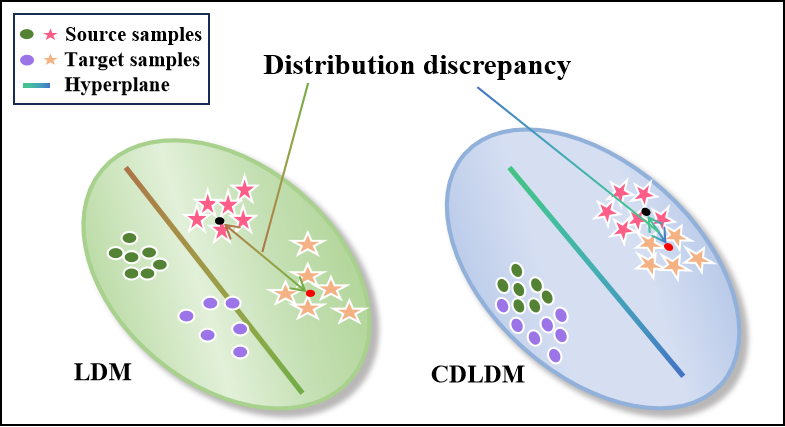
\includegraphics[height=0.2\textheight, width=0.48\textwidth]{CDLDM3.png}
    \caption{CDLDM method schematic. LDM does not consider the distribution discrepancy of data, which makes it difficult for the classifier learned in the source domain to generalize effectively to the target domain. The proposed CDLDM aims to overcome this shortcoming of LDM. It is observed that when the distribution of source domain and target domain tends to be the same, the classifier learned from the source domain can be more effectively applied to the target domain.}
    \label{CDLDM}
\end{figure}

\section{Proposed Methodology}\label{novel}
In this section, we first provide a notation explanation in Section \ref{not}. Then, a novel efficient Cross-Domain Large Margin Distribution Machine is presented in Section \ref{MODEL}. As shown in Fig. \ref{CDLDM}, the proposed CDLDM is intended minimize the global distribution discrepancy of data. 
Finally, the pseudocode for the CDLDM algorithm is outlined in Section \ref{time}.



\subsection{Notations}\label{not}
In the field of machine learning, a domain $\mathcal{D}$ consists of a feature space $\mathcal{\boldsymbol{X}}$ and a marginal probabilistic distribution $P(\boldsymbol{\boldsymbol{X}})$ on the feature space, i.e., $\mathcal{D} = \{ \mathcal{\boldsymbol{X}},\ P(\boldsymbol{\boldsymbol{X}})\}$, where $\boldsymbol{\boldsymbol{X}} = \boldsymbol{\boldsymbol{x_i}}_{i=1}^m \in \mathcal{\boldsymbol{X}}$.
After giving a domain $\mathcal{D} = \{ \mathcal{\boldsymbol{X}},\ P(\boldsymbol{\boldsymbol{X}})\}$,
% a task $\mathcal{T}$ is composed of a label space $\boldsymbol{Y}$ and an objective prediction function $f(.)$, i.e., $\mathcal{T}=\{\boldsymbol{Y}, f(.)\}$, 
a task $\mathcal{T}$ consists of a label $\boldsymbol{Y}$ and an objective prediction function $f(.)$, represented as $\mathcal{T} = \{\boldsymbol{Y}, f(.)\}$. The objective prediction function $f(.)$ cannot be directly observed, but can be learned from training data composed of feature label pairs $(\boldsymbol{x_i}\in \boldsymbol{X}, y_i\in Y)$. From the perspective of probability theory, the objective prediction function $f(.)$ can be expressed as $P (Y | \boldsymbol{X})$. The task is represented as $\mathcal{T}=\{Y, P (Y | \boldsymbol{X})\}$. In the problem of E-nose drift, there are two crucial concepts: The source domain represents as $\mathcal{D}_{S} = \{(\boldsymbol{X_S}^{1},y_{S}^{1}),\ldots,(\boldsymbol{X_S}^{m},y_{S}^{m})\}$ and the target domain represents $\mathcal{D}_{T} = \{(\boldsymbol{x_{T}}^{1},y_{T}^{1}),\ldots,(\boldsymbol{x_{T}^{n}},y_{T}^{n})\}$. The data of the source and target domains are represented as $\boldsymbol{X_S} = [\boldsymbol{X_S}^{1},\ldots,\boldsymbol{X_S}^{m}]\in \mathcal{R}^{D\times N_S}$ with corresponding labels $\boldsymbol{Y_S} = [y_{S}^{1},\ldots,y_{S}^{n}]\in \mathcal{R}^{D\times C}$ and $\boldsymbol{X_T} = [\boldsymbol{x_{T}}^{1},\ldots,\boldsymbol{x_{T}}^{n}]\in \mathcal{R}^{D\times N_T}$ with corresponding labels $\boldsymbol{Y_T} = [y_{T}^{1},\ldots,y_{T}^{n}]\in \mathcal{R}^{D\times C}$, where $D$ represents the feature dimensionality, and $C$ indicates the overall count of categories.
% $N_S = m$ and $N_T = n$ represents the number of samples in the source and target domains, respectively. The source domain and target domain often belong to the same type of task, but their distribution is different, i.e., $P_S(\boldsymbol{X_S},\boldsymbol{Y_S}) \neq P_T(X_T,Y_T)$.
% The quantity of samples in the source domain is denoted as $N_S = m$, 
$N_S = m$ denotes the number of samples in the source domain, while in the target domain, it is represented as $N_T = n$. Although the source and target domains typically pertain to the same type of task, their data distributions exhibit distinct characteristics, i.e., $P_S(\boldsymbol{X_S},\boldsymbol{Y_S}) \neq P_T(X_T,Y_T)$.



\subsection{Cross-Domain LDM} \label{MODEL}
In this section, we elaborate on the methodology for constructing the model, as detailed in Section \ref{construction}.
The measure of the projection distribution discrepancy is shown in detail in Section \ref{measure}. Finally, Section \ref{optimization} presents the optimization procedure.

\subsubsection{Model construction of CDLDM}\label{construction}
LDM is a widely used algorithm. Its core idea is to obtain better generalization performance by optimizing the margin distribution. For a hyperplane classifier like LDM, the decision function is expressed as $f(\boldsymbol{x}) = \boldsymbol{\omega}^\mathrm{T}\boldsymbol{x}+b$, where $\boldsymbol{\omega}$ is a normal projection vector and $b$ is the offset. 
Conventional machine learning paradigms typically presuppose that the training and test datasets adhere to an identical distribution, i.e., $P_s(\boldsymbol{X_S},\boldsymbol{Y_S}) = P_t(X_T,Y_T)$. In this case, traditional LDM performs well. However, in many cases, this same distribution assumption is not satisfied, i.e., $P_S(\boldsymbol{X_S},\boldsymbol{Y_S}) \neq P_t(X_T,Y_T)$. The drift caused by gas sensors in E-nose systems is precisely such a situation. Hence, in addressing the challenge of E-noses drift, our objective is to identify a feature transformation, $f(\boldsymbol{x}) = \boldsymbol{\omega}^\mathrm{T} \phi(\boldsymbol{x})$, within a universal RKHS that effectively reduce the discrepancy between the data distributions of the two domains, thereby achieving cross-domain learning. Drawing inspiration from the concept of Manifold Regularization \citep{belkin2006manifold}, we can formulate the optimization problem of CDLDM as follows
\begin{equation}
\label{cdldm1}
\begin{aligned}
&f = \min _{\boldsymbol{\omega}\ \in H_K} \ C \sum_{i=1}^{m} V(\boldsymbol{x_i},\ y_{i},\ f)+\frac{1}{2}{\|f\|}_{K}^{2} \\
&+\lambda_1\widehat \gamma - \lambda_2\bar \gamma+\lambda D_{g}(\boldsymbol{X_S},\ X_T),
\end{aligned}
\end{equation}
where $V$ represents the risk function. 
% $K$ denotes a kernel equipped with a kernel mapping function, $H_K$ is a set of functions in the kernel space.
$K$ refers to a kernel with its associated mapping function. 
% The set $H_K$ includes all functions that belong to the kernel space.
${\|f\|}_{K}^{2}$ is the $L_2$ norm of the function $f$. The loss function adopts the hinge loss function used by traditional LDM, which is represented as $V = (1-y_if(\boldsymbol{x_i}))_+$, where $(x)_+ = x\ if\ x\geq 0$ and 0 otherwise. Hence, Eq. (\ref{cdldm1}) can be further represented by the given function $f(\boldsymbol{x}) = \textless\boldsymbol{\omega},\phi(\boldsymbol{x})\textgreater_H$ as
\begin{equation}\label{cdldm2}
\begin{aligned}
&f = \min _{\boldsymbol{\omega} \in H_K} \ \frac{1}{2}\boldsymbol{\omega}^{\mathrm{T}}\boldsymbol{\omega} + \lambda_1\widehat \gamma - \lambda_2\bar \gamma + C\sum\limits_{i = 1}^m\xi_i + \lambda D_{g}(\boldsymbol{X_S},\ \boldsymbol{X_T}), \\
& s.t.\ y_{i}\boldsymbol{\omega}^{\mathrm{T}}\phi(\boldsymbol{x_i})\geq 1-\xi_{i},\\
&\ \quad \xi_{i} \geq 0,\quad i=1,2, \ldots, m,
\end{aligned}    
\end{equation}
where $\boldsymbol{x_i} \in \boldsymbol{X_S}$ and $H$ represents the complete inner product space for $f$. And $D_{g}(\boldsymbol{X_S},\ X_T)$ is a measure of the projection distribution discrepancy, specifically represented as follows
\begin{equation}
D_{g}(\boldsymbol{X_S},\ X_T) = \lambda_3 D_f + \lambda_4 S_f + \lambda_5 P_f,
\end{equation}
% where $D_f$ represents the projection marginal distribution discrepancy on the distribution of RKHS embedding domains, $S_f$ indicates the projection scattering distribution discrepancy on the RKHS embedding domain, and $P_f$ is the graph-based Laplacian regularization.
where, $D_f$ denotes the discrepancy in the projection marginal distribution of RKHS embedding domains, $S_f$ represents the discrepancy in the projection scattering distribution on these domains, and $P_f$ refers to the graph-based Laplacian regularization.

% Fortunately, inspired by the representer theorem in [], $f \in H$ can be expressed as 
% \begin{equation}
%     f(x) = \sum_{i=1}^m \alpha_i k(\boldsymbol{x_i},x) + \sum_{j=1}^n \alpha_{j+m} k(\boldsymbol{z_j},x)
% \end{equation}
% where $\boldsymbol{x_i} \in \boldsymbol{X_S}$, $\boldsymbol{z_j} \in X_T$, and $k$ is the kernel function and $\boldsymbol{\alpha} = [\alpha_1,\ldots,\alpha_m,\ldots,\alpha_{m+n}]^{\mathrm{T}}$ are the specific coefficients. Furthermore, we can express $\boldsymbol{\omega}$ in kernel space as
% \begin{equation}\label{omega}
% \boldsymbol{\omega} = \phi(\boldsymbol{X_{st}})\boldsymbol{\alpha} = \sum_{i=1}^m \alpha_i \phi(\boldsymbol{x_i}) + \sum_{j=1}^n \alpha_{j+m} \phi(\boldsymbol{z_j})
% \end{equation}
% where $\boldsymbol{X_{st}} = ({\boldsymbol{x_i}}_{i=1}^m,{\boldsymbol{z_j}}_{j=1}^n)$. Furthermore,***

% ---------------------remark1:degenerates----------------------

\begin{remark}
The CDLDM is a universal framework that can  degenerate into conventional models as needed.


\begin{itemize}
\item[$\bullet$] When $\lambda = 0$, the CDLDM model reverts to LDM. This study marks the first instance of extending the LDM model to the domain of cross-domain learning, addressing the real-world challenge of knowledge transfer across multiple domains. While traditional LDM primarily focuses on learning within a single domain, practical applications frequently involve the problem of knowledge transfer between multiple domains, i.e., how to effectively apply knowledge and experience acquired in one domain to others. The introduction of the CDLDM model aims to tackle this complex challenge.

\item[$\bullet$] When $\lambda, \lambda_1, \lambda_2 = 0$, the CDLDM model degenerates into SVM. CDLDM enhances the architecture of SVM by optimizing the marginal distribution and extending it to cross-domain domains.
Specifically, the CDLDM model aims to improve the generalization ability and performance of the model by optimizing the marginal distribution. By minimizing feature differences between different domains, the model's adaptability in different domains is further enhanced.
Overall, these improvements enable the model to better adapt to different domains of data and enhance its performance in practical applications.
\end{itemize}
\end{remark}

Incorporating Eqs. (\ref{mean}) and (\ref{variance}) into Eq. (\ref{cdldm2}), we can derive the quadratic programming problem as follows
\begin{equation}\label{cdldm3}
\begin{aligned}
&\mathop {\min }\limits_{\boldsymbol{\omega},\ \xi } f = \ \frac{1}{2}\boldsymbol{\omega}^{\mathrm{T}}\boldsymbol{\omega} + \frac{2\lambda_1}{m^2}(m\boldsymbol{\omega}^{\mathrm{T}}\phi(\boldsymbol{X_S})\phi(\boldsymbol{X_S})^{\mathrm{T}}\boldsymbol{\omega} \\
&- \boldsymbol{\omega}^{\mathrm{T}}\phi(\boldsymbol{X_S})\boldsymbol{Y_S}\boldsymbol{Y_S}^{\mathrm{T}}\phi(\boldsymbol{X_S})^{\mathrm{T}}\boldsymbol{\omega}) - \lambda_2\frac{1}{m}(\phi(\boldsymbol{X_S})\boldsymbol{Y_S})^{\mathrm{T}}\boldsymbol{\omega}\\
&+ C\sum\limits_{i = 1}^m\xi_i + \lambda D_{g}(\boldsymbol{X_S},\ X_T), \\
& s.t.\ y_{i}\boldsymbol{\omega}^{\mathrm{T}}\phi(\boldsymbol{x_i})\geq 1-\xi_{i},\\
&\ \ \quad \xi_{i} \geq 0,\quad i=1,2, \ldots, m.
\end{aligned}    
\end{equation}

Eq. (\ref{cdldm3}) is usually difficult to handle. According to the representation theorem in \cite{belkin2006manifold}, we can rephrase Eq. (\ref{cdldm3}) using the following Representer theorem.

% ----------------------myTheo1:omega-------------------------

\begin{myTheo}\label{theo1}
 The optimal solution $\boldsymbol{\omega}$ of Eq. (\ref{cdldm3}) can be succinctly expressed as 
\begin{equation}\label{omega}
\boldsymbol{\omega} = \phi(\boldsymbol{X_{st}})\boldsymbol{\alpha} = \sum_{i=1}^m \alpha_i \phi(\boldsymbol{x_i}) + \sum_{j=1}^n \alpha_{j+m} \phi(\boldsymbol{z_j})
\end{equation}
where $\boldsymbol{x_i} \in \boldsymbol{X_S}$, $\boldsymbol{z_j} \in X_T$, $\boldsymbol{X_{st}} = ({\boldsymbol{x_i}}_{i=1}^m,{\boldsymbol{z_j}}_{j=1}^n)$, and $\boldsymbol{\alpha} = [\alpha_1,\ldots,\alpha_m,\ldots,\alpha_{m+n}]^{\mathrm{T}}$ are the specific coefficients.
\end{myTheo}
\begin{proof}
Due to the correlation between the projection vector $\boldsymbol{\omega}$ and both the source and target samples, $\boldsymbol{\omega}$ can be decomposed into a part that exists within the span of $\phi(\boldsymbol{x_i})$ and $\phi(\boldsymbol{z_j})$ and an orthogonal part vector, i.e.,
\begin{equation}
\boldsymbol{\omega}  = \sum_{i=1}^m \alpha_i \phi(\boldsymbol{x_i}) + \sum_{j=1}^n \alpha_{j+m} \phi(\boldsymbol{z_j}) + \boldsymbol{\beta}= \phi(\boldsymbol{X_{st}})\boldsymbol{\alpha} +\boldsymbol{\beta},
\end{equation}
where $\boldsymbol{\beta}$ denotes a vector  that adheres to the condition $\phi(\boldsymbol{X_{st}})\boldsymbol{\beta} = 0$ \cite{zhang2014large}. Then, we have
\begin{equation}
\phi(\boldsymbol{X_S})^\mathrm{T} \boldsymbol{\omega} = \phi(\boldsymbol{X_S})^\mathrm{T} (\phi(\boldsymbol{X_{st}})\boldsymbol{\alpha} +\boldsymbol{\beta}) = \phi(\boldsymbol{X_S})^\mathrm{T} \phi(\boldsymbol{X_{st}}) \boldsymbol{\alpha},
\end{equation}
so the second and the third terms in the (\ref{cdldm3}) are unrelated to $\boldsymbol{\beta}$, and the fourth term is independent of $\boldsymbol{\beta}$. Additionally, the constraint is also not correlated with $\boldsymbol{\beta}$. For the first term and last terms related to $\boldsymbol{\beta}$ in the (\ref{cdldm3}), according to $\phi(\boldsymbol{X_{st}})\boldsymbol{\beta} = 0$, we can obtain (only the first term is extrapolated here, and the last term is the same)
\begin{equation}
\begin{aligned}
\boldsymbol{\omega}^\mathrm{T} \boldsymbol{\omega} & = (\phi(\boldsymbol{X_{st}})\boldsymbol{\alpha} +\boldsymbol{\beta})^\mathrm{T} (\phi(\boldsymbol{X_{st}})\boldsymbol{\alpha} +\boldsymbol{\beta})\\
& = \boldsymbol{\alpha}^\mathrm{T} \phi(\boldsymbol{X_{st}})^\mathrm{T} \phi(\boldsymbol{X_{st}}) \boldsymbol{\alpha} + \boldsymbol{\beta}^\mathrm{T} \boldsymbol{\beta}\\
& \geq \boldsymbol{\alpha}^\mathrm{T} \phi(\boldsymbol{X_{st}})^\mathrm{T} \phi(\boldsymbol{X_{st}}) \boldsymbol{\alpha},
\end{aligned}
\end{equation}
where if and only if $\boldsymbol{\beta} = 0$, the equal sign holds.

Therefore, the $\boldsymbol{\beta}$ setting to 0 does not influence the second, third, and fourth terms, but strictly reduces the first and last items of (\ref{cdldm3}). Hence, Theorem \ref{theo1} is accepted.
\end{proof}

% % ---------------------remark1:degenerates----------------------

% \begin{remark}
% CDLDM is a general model, and we have the following empirical findings. 
% \begin{itemize}
% \item[$\bullet$] When $\lambda = 0$, the CDLDM model reverts to the traditional LDM. This study marks the first instance of extending the LDM model to the domain of cross-domain learning, addressing the real-world challenge of knowledge transfer across multiple domains. While traditional LDM primarily focuses on learning within a single domain, practical applications frequently involve the problem of knowledge transfer between multiple domains, i.e., how to effectively apply knowledge and experience acquired in one domain to others. The introduction of the CDLDM model aims to tackle this complex challenge.

% \item[$\bullet$] When $\lambda, \lambda_1, \lambda_2 = 0$, the CDLDM model degenerates into traditional SVM. The proposed model modifies the structure of SVM by optimizing the marginal distribution and extending it to cross-domain domains.
% Specifically, the CDLDM model aims to improve the generalization ability and performance of the model by optimizing the marginal distribution. By minimizing feature differences between different domains, the model's adaptability in different domains is further enhanced.
% Overall, these improvements enable the model to better adapt to different fields of data and enhance its performance in practical applications.
% \end{itemize}
% \end{remark}

\subsubsection{The measure of projection distribution discrepancy}\label{measure}
In this section, we provide a detailed introduction to the projection marginal distribution discrepancy $D_f$, the projection scattering distribution discrepancy $S_f$, and the graph-based Laplacian regularization $P_f$.

% ---------Projected Marginal Distribution Discrepancy--------

\textbf{ 1) Projected Marginal Distribution Discrepancy}

In the context of E-noses drift issues, our primary objective is to mitigate the differences in data distributions across various domains by means of learning a feature transformation. Consequently, the effective measurement of distribution disparities between domains becomes a paramount concern. In this pursuit, it is crucial to select a method suitable for quantifying distribution dissimilarity, while ensuring that the chosen method is computationally efficient and easily integrated into the optimization problem of LDM. Maximum Mean Discrepancy (MMD) has been demonstrated as an effective approach for estimating the distance between two distributions, offering a relatively straightforward implementation with fast computation speed. 
% Hence, we employ the MMD metric to estimate the distribution discrepancy between two domains in a universal RKHS. 
Therefore, we utilize the MMD metric to measure the distribution differences.
The $D_f$ is defined as
\begin{equation}\label{Df}
\begin{aligned}
&D_{f}\left(\boldsymbol{X_S}, \boldsymbol{X_T}\right) \\
&=  \boldsymbol{\omega}^{\mathrm{T}}\left\|\frac{1}{m} \sum_{i=1}^{m} \phi\left(\boldsymbol{x_i}\right)-\frac{1}{n} \sum_{j=1}^{n} \phi\left(\boldsymbol{z_j}\right)\right\|_{\mathcal{H}}^{2} \boldsymbol{\omega} \\
&=  \left\|\frac{1}{m} \sum_{k=1}^{m+n} \alpha_{k}^{\mathrm{T}} \phi\left(\boldsymbol{x_k}\right)^{\mathrm{T}} \sum_{i=1}^{m} \phi\left(\boldsymbol{x_i}\right)\right. \left.-\frac{1}{n} 
\sum_{k=1}^{m+n} \alpha_{k}^{\mathrm{T}} \phi\left(\boldsymbol{x_k}\right)^{\mathrm{T}} \sum_{j=1}^{n} \phi\left(\boldsymbol{z_j}\right)\right\|^{2} \\
&=  \frac{1}{m^{2}} \sum_{k, l=1}^{m+n} \alpha_{k}^{\mathrm{T}} \phi\left(\boldsymbol{x_k}\right)^{\mathrm{T}} \sum_{i=1}^{m} \phi\left(\boldsymbol{x_i}\right) \sum_{j=1}^{m} \phi\left(\boldsymbol{x_j}\right) \phi\left(\boldsymbol{x_l}\right) \alpha_{l} \\
 &+\frac{1}{n^{2}} \sum_{k, l=1}^{m+n} \alpha_{k}^{\mathrm{T}} \phi\left(\boldsymbol{x_k}\right)^{\mathrm{T}} \sum_{i=1}^{n} \phi\left(z_{i}\right) \sum_{j=1}^{n} \phi\left(\boldsymbol{z_j}\right) \phi\left(\boldsymbol{x_l}\right) \alpha_{l}\\
& -\frac{1}{m n}\left(\sum_{k, l=1}^{m+n} \alpha_{k}^{\mathrm{T}} \phi\left(\boldsymbol{x_k}\right)^{\mathrm{T}} \sum_{i=1}^{m} \phi\left(\boldsymbol{x_i}\right) \sum_{j=1}^{n} \phi\left(\boldsymbol{z_j}\right) \phi\left(\boldsymbol{x_l}\right) \alpha_{l}\right. \\
& \left.-\sum_{k, l=1}^{m+n} \alpha_{k}^{\mathrm{T}} \phi\left(\boldsymbol{x_k}\right)^{\mathrm{T}} \sum_{j=1}^{n} \phi\left(\boldsymbol{z_j}\right) \sum_{i=1}^{m} \phi\left(\boldsymbol{x_i}\right) \phi\left(\boldsymbol{x_l}\right) \alpha_{l}\right) \\
&=  \boldsymbol{\alpha}^{\mathrm{T}}\left(\frac{1}{n^{2}} \boldsymbol{K_{{S}}}\boldsymbol{[1]}^{m \times m} \boldsymbol{K_{S}}^{\mathrm{T}}+\frac{1}{m^{2}} K_{{T}}\boldsymbol{[1]}^{n \times n} \boldsymbol{K_{T}}^{\mathrm{T}}\right. \\
& \left.-\frac{1}{n m}\left(\boldsymbol{K_{{S}}}\boldsymbol{[1]}^{m \times n} \boldsymbol{K_{{T}}}^{\mathrm{T}}+\boldsymbol{K_{{T}}}\boldsymbol{[1]}^{n \times m} \boldsymbol{K_{{S}}}^{\mathrm{T}}\right)\right) \boldsymbol{\alpha} \\
&=  \boldsymbol{\alpha}^{\mathrm{T}} \boldsymbol{\Omega}_{d} \boldsymbol{\alpha},
\end{aligned}
\end{equation}
where $\boldsymbol{[1]}^{m \times m}$ represents a $m \times m$ matrix of all ones. $\boldsymbol{K_S}\in \mathbb{R}^{(m+n) \times m}$ and $\boldsymbol{K_T}\in \mathbb{R}^{(m+n) \times n}$ is the kernel matrix for the source samples and the target samples, respectively. $\Omega_d$ is a
$(m + n) \times (m + n)$ symmetrical positive semi-definite kernel matrix, which is defined as
\begin{equation}
\begin{aligned}
&\Omega_d = \frac{1}{n^{2}} \boldsymbol{K_{{S}}}\boldsymbol{[1]}^{m \times m} \boldsymbol{K_{S}}^{\mathrm{T}}+\frac{1}{m^{2}} K_{{T}}\boldsymbol{[1]}^{n \times n} \boldsymbol{K_{T}}^{\mathrm{T}} \\
& -\frac{1}{n m}\left(\boldsymbol{K_{{S}}}\boldsymbol{[1]}^{m \times n} \boldsymbol{K_{{T}}}^{\mathrm{T}}+\boldsymbol{K_{{T}}}\boldsymbol{[1]}^{n \times m} \boldsymbol{K_{{S}}}^{\mathrm{T}}\right).
\end{aligned}
\end{equation}

% -------Projection Scattering Distribution Discrepancy------

\textbf{2) Projection Scattering Distribution Discrepancy}

In order to effectively assess the distribution differences between the source domain and the target domain, we need to consider the variance or dispersion of the data. This is particularly important because dispersion reflects the degree of spread of data points within the distribution, providing crucial information about the breadth and tightness of the data distribution. 
Therefore, it is necessary to make full use of the scatter information from source and target domains in order to comprehensively assess distribution differences. 
The $S_f$ is defined as
\begin{equation}\label{Sf}
\begin{aligned}
&S_f \left({\boldsymbol{X}}_{s}, {\boldsymbol{X}}_{T}\right) \\
& ={\boldsymbol{\omega}}^\mathrm{T}\left|\frac{1}{m} \sum_{i=1}^{m} \phi\left(\boldsymbol{x_i}\right) \phi\left(\boldsymbol{x_i}\right)^\mathrm{T}-\frac{1}{n} \sum_{j=1}^{n} \phi\left(\boldsymbol{z_j}\right)\phi\left(\boldsymbol{z_j}\right)^\mathrm{T}\right|_{\mathcal{H}} {\boldsymbol{\omega}} \\
& =\left| \frac{1}{m} \sum_{j, k}^{m+n} \alpha_{j}^\mathrm{T} \phi\left(\boldsymbol{x_j}\right)^\mathrm{T} \sum_{i=1}^{m} \phi\left(\boldsymbol{x_i}\right)\phi\left(\boldsymbol{x_i}\right)^\mathrm{T} \alpha_{k} \phi\left(\boldsymbol{x_k}\right) \right.\\
& - \left. \frac{1}{n} \sum_{j, k}^{m+n} \alpha_{j}^\mathrm{T} \phi\left(\boldsymbol{x_j}\right)^\mathrm{T} \sum_{i=1}^{n} \phi\left(\boldsymbol{z_i}\right)\phi\left(\boldsymbol{z_i}\right)^\mathrm{T} \alpha_{k} \phi\left(\boldsymbol{x_k}\right) \right| \\
& =\left| \frac{1}{m} \sum_{j, k}^{m+n} \alpha_{j}^\mathrm{T} \alpha_{k} \sum_{i=1}^{m} k\left(\boldsymbol{x_j}, \boldsymbol{x_i}\right) k\left(\boldsymbol{x_i}, \boldsymbol{x_k}\right) \right. \\
& - \left. \frac{1}{n} \sum_{j, k}^{m+n} \alpha_{j}^\mathrm{T} \alpha_{k} \sum_{i=1}^{n} k\left(\boldsymbol{x_j}, \boldsymbol{z_i}\right) k\left(\boldsymbol{z_i}, \boldsymbol{x_k}\right) \right| \\
& ={\boldsymbol{\alpha}}^\mathrm{T}\left|\frac{1}{m} \boldsymbol{K_S} \boldsymbol{K_S}^\mathrm{T}-\frac{1}{n} \boldsymbol{K_T} \boldsymbol{K_T}^\mathrm{T}\right| {\boldsymbol{\alpha}}={\boldsymbol{\alpha}}^\mathrm{T} {\boldsymbol{\Omega}}_{s} {\boldsymbol{\alpha}},
\end{aligned}
\end{equation}
where $\boldsymbol{\Omega_s}$ is a
$(m + n) \times (m + n)$ symmetrical positive semi-definite kernel matrix, which is defined as
\begin{equation}
\boldsymbol{\Omega_s} = \left|\frac{1}{m} \boldsymbol{K_S} \boldsymbol{K_S}^\mathrm{T}-\frac{1}{n} \boldsymbol{K_T} \boldsymbol{K_T}^\mathrm{T}\right|.
\end{equation}

% -------Graph-based Laplacian regularization--------------
\textbf{3) Graph-based Laplacian regularization}

Manifold theory suggests that samples near each other in the original sample space will also be close in the projected RKHS, indicating a higher likelihood of belonging to the same class. Thus, in the context of E-nose data analysis, it is reasonable to consider that samples that are close together in the original feature space are probably from the same class. In order to maintain the geometric relationship between samples in RKHS, we added a graph-based Laplacian regularization term to the optimization function of CDLDM. The $P_f$ is defined as 
\begin{equation}\label{Pf}
\begin{aligned}
&P_{f}\left(X_{{S}}, X_{T}\right) \\
& =\boldsymbol{\omega}^{\mathrm{T}}\left\|\sum_{i, j=1}^{m+n} W_{ij} \left(f\left(\boldsymbol{x_i}\right)-f\left(\boldsymbol{x_j}\right)\right)^{2}\right\|_{\mathcal{H}} \boldsymbol{\omega} \\
& =\sum_{k=1}^{m+n} \alpha_{k}^{\mathrm{T}} \phi\left(\boldsymbol{x_k}\right)^{\mathrm{T}} \sum_{i, j=1}^{m+n} \phi\left(\boldsymbol{x_i}\right) L_{i j} \phi\left(\boldsymbol{x_j}\right) \sum_{l=1}^{m+n} \alpha_{l} \phi\left(\boldsymbol{x_l}\right) \\
& ={\boldsymbol{\alpha}}^{\mathrm{T}} \boldsymbol{K_{st}} \boldsymbol{L} \boldsymbol{K_{st}}^{\mathrm{T}} {\boldsymbol{\alpha}} \\
& ={\boldsymbol{\alpha}}^{\mathrm{T}} {\boldsymbol{\Omega}}_{{p}} {\boldsymbol{\alpha}},
\end{aligned}
\end{equation}
where $\boldsymbol{K_{st}} \in \mathbb{R}^{(m+n) \times (m+n)}$ is the kernel matrix for samples in $X_{st}$, $\boldsymbol{\Omega_{p}} = \boldsymbol{K_{st}} \boldsymbol{L} \boldsymbol{K_{st}}^{\mathrm{T}} $. $\boldsymbol{W}$ is the proximity relationship matrix between samples, which is defined as
\begin{equation}
W_{ij} = \begin{cases}1 & x_i \in N_{p}(x_j)\ or\ x_j \in N_{p}(x_i) \\ 0 & {\text {otherwise}}\end{cases},
\label{p}
\end{equation}
where $N_{p}(x_i)$ is the sets of the $p-$nearest neighbors of $x_i$. $\boldsymbol{L}$ is the graph Laplacian matrix and is computed as $\boldsymbol{L} = \boldsymbol{D} - \boldsymbol{W}$, $D$ is a diagonal matrix with $D_{ij} = \sum\nolimits_{j=1}^{m+n} W_{ij}$.


\subsubsection{Model Optimization}\label{optimization}
In sections \ref{measure}, we obtain the specific representation of the measurement of the projection distribution discrepancy in RHKS through $D_f, S_f$, and $P_f$, which can be further represented as
\begin{equation}\label{D_g}
\begin{aligned}
D_g &= \lambda_3 D_f + \lambda_4 S_f + \lambda_5 P_f \\
&= \boldsymbol{\alpha}^{\mathrm{T}}(\lambda_3 \boldsymbol{\Omega}_d + \lambda_4 \boldsymbol{\Omega}_s +\lambda_5 \boldsymbol{\Omega}_p)\boldsymbol{\alpha} \\
&= \boldsymbol{\alpha}^{\mathrm{T}} \boldsymbol{\Omega}_{g}\ \boldsymbol{\alpha},
\end{aligned}
\end{equation}
where $\boldsymbol{\Omega}_g = \lambda_3 \boldsymbol{\Omega}_d + \lambda_4 \boldsymbol{\Omega}_s +\lambda_5 \boldsymbol{\Omega}_p$ is a $(n+m) \times (n+m)$ positive  semi-definite kernel matrix.

% ----------------------myTheo2: optimization--------------------

\begin{myTheo}\label{QPP}
The dual formulation of the initial problem stated in Eq. (\ref{cdldm2}) is expressed below
\begin{equation}
\begin{aligned}
\label{end}
&\mathop {\min } \limits_{\boldsymbol{\eta}} f= \quad {\rm{   }}\frac{1}{2}{\boldsymbol{\eta}^{\mathrm{T}}}\boldsymbol{M}\boldsymbol{\eta} + {(\frac{{{\lambda _2}\boldsymbol{M}\boldsymbol{e} - m\boldsymbol{e}}}{m})^{\mathrm{T}}}\boldsymbol{\eta}, \\
& s.t.\quad  0 \le \eta_i  \le {C} ,\ i = 1,...,m,
\end{aligned}
\end{equation}
\end{myTheo}

\begin{proof}
Drawing from Theorem \ref{theo1}, we can infer the subsequent expressions
\begin{equation}\label{oo}
\begin{aligned}
&\boldsymbol{\omega}^{\mathrm{T}} \phi(\boldsymbol{X_S}) = \boldsymbol{\alpha}^{\mathrm{T}} \phi(\boldsymbol{X_{st}})^{\mathrm{T}} \phi(\boldsymbol{X_S})  =\boldsymbol{\alpha}^{\mathrm{T}} \boldsymbol{K_S} ,\\
&\boldsymbol{\omega}^{\mathrm{T}} \boldsymbol{\omega} = \boldsymbol{\alpha}^{\mathrm{T}} \phi(\boldsymbol{X_{st}})^{\mathrm{T}} \phi(\boldsymbol{X_{st}}) \boldsymbol{\alpha} = \boldsymbol{\alpha}^{\mathrm{T}} \boldsymbol{G} \boldsymbol{\alpha},
\end{aligned}
\end{equation}
where $\boldsymbol{K_S} = \phi(\boldsymbol{X_{st}})^{\mathrm{T}} \phi(\boldsymbol{X_S})$ and $\boldsymbol{G} =\phi(\boldsymbol{X_{st}})^{\mathrm{T}} \phi(\boldsymbol{X_{st}}) $ are the kernel matrix. Let $\boldsymbol{\boldsymbol{K_{:i}}}$ represent the $i-$th column of $\boldsymbol{K_S}$.

Substituting Eqs. (\ref{D_g}) and (\ref{oo}) into Eq. (\ref{cdldm3}), the matrix form of the CDLDM can be obtained
\begin{equation}
\begin{aligned}
\label{matrix}
&\mathop {\min }\limits_{\boldsymbol{\alpha},\ \xi } f = \ \ \frac{1}{2}{\boldsymbol{\alpha} ^{\mathrm{T}}}\boldsymbol{Q}\boldsymbol{\alpha}  + {\boldsymbol{q}^{\mathrm{T}}}\boldsymbol{\alpha}  + C \sum\limits_{i = 1}^m {{\xi _i}}, \\
& s.t.  \quad y_{i}\boldsymbol{\alpha}^{\mathrm{T}} \boldsymbol{\boldsymbol{K_{:i}}} \geq 1-\xi_{i}, \ \ i=1,2, \ldots, m,\\
&\ \quad\ \ \  \  \xi_{i} \geq 0,\quad i=1,2, \ldots, m,
\end{aligned}
\end{equation}
where ${\boldsymbol{Q}  = 4}{\lambda _1}(m \boldsymbol{K_S} {\boldsymbol{K_S}^{\mathrm{T}}} - (\boldsymbol{K_S} \boldsymbol{Y_S}){(\boldsymbol{K_S} \boldsymbol{Y_S})^{\mathrm{T}}})/{m^2} + \boldsymbol{G} +2 \boldsymbol{\Omega}_{g}$  and $\boldsymbol{q}= - {\lambda _2}\boldsymbol{K_S} \boldsymbol{Y_S}/m$. 

% --------------------------kkt-----------------------------
The Lagrangian formulation corresponding to the optimization problem delineated in Eq. (\ref{matrix}) is articulated as follows
% The Lagrangian function of model (\ref{matrix}) is presented as
\begin{equation}
\begin{aligned}
\label{laa}
&L(\boldsymbol{\alpha}, \xi ;\boldsymbol{\eta}, \delta ) = \frac{1}{2}{\boldsymbol{\alpha} ^{\mathrm{T}}}\boldsymbol{Q}\boldsymbol{\alpha}  + {\boldsymbol{q}^{\mathrm{T}}}\boldsymbol{\alpha}  + C \sum\limits_{i = 1}^m {{\xi _i}} \\
 &- \sum\limits_{i = 1}^m {{{\eta} _i}({\xi _i} + {y_i}{\boldsymbol{\alpha} ^{\mathrm{T}}}{ \boldsymbol{\boldsymbol{K_{:i}}}} - 1)}- \sum\limits_{i = 1}^m {{\delta _i}{\xi _i}},
\end{aligned}
\end{equation}
where $\boldsymbol{\eta}\ and\ \boldsymbol{\delta}$ are Lagrangian vectors. Let $\partial {L}/\partial {\alpha } = \partial {L}/\partial {\xi }_{i} = 0$, we obtain the following formulas
% By setting the partial derivations of $\{ \boldsymbol{\alpha},\boldsymbol{\xi} \}$ to \{0\}, we derive the following equations
\begin{equation}
\begin{array}{l}
\label{kkt}
\frac{{\partial {L}}}{{\partial \boldsymbol{\alpha} }} = \boldsymbol{Q}\boldsymbol{\alpha}  + \boldsymbol{q} - \sum\limits_{i = 1}^m {{{\eta} _i}{y_i}{ \boldsymbol{\boldsymbol{K_{:i}}}}  }  = 0,\\
\frac{{\partial {L}}}{{\partial {\xi _i}}} = C - {{\eta} _i} - {\delta _i} = 0, 
\end{array}
\end{equation}
% ------------------------final dual------------------------
introduced Eq. (\ref{kkt}) into Eq. (\ref{laa}), the dual form of model (\ref{matrix}) is exhibited as follow
\begin{equation}
\begin{aligned}
\label{end}
&\mathop {\min } \limits_{\boldsymbol{\eta}} f= \quad {\rm{   }}\frac{1}{2}{\boldsymbol{\eta}^{\mathrm{T}}}\boldsymbol{M}\boldsymbol{\eta} + {(\frac{{{\lambda _2}\boldsymbol{M}\boldsymbol{e} - m\boldsymbol{e}}}{m})^{\mathrm{T}}}\boldsymbol{\eta}, \\
& s.t.\quad  0 \le \eta_i  \le {C} ,\ i = 1,...,m,
\end{aligned}
\end{equation}
where $\boldsymbol{M}=[diag(\boldsymbol{Y_S})] \boldsymbol{K_S} {\boldsymbol{Q}^{ - 1}}\boldsymbol{K_S}[diag(\boldsymbol{Y_S})]$, $\boldsymbol{e} = {[1,...,1]_{1 \times m}}$.
\end{proof}

% -----------------myTheo3:decison function----------------
% \begin{myTheo}
% By utilizing Theorem \ref{QPP}, we obtained the dual problem of the original problem. Then, a decision function for CDLDM can be derived to tackle data classification problems
% \end{myTheo}

% \begin{proof}

Based on Eq. (\ref{kkt}), the parameter $\boldsymbol{\alpha}$ can be determined using the subsequent expression
\begin{equation}\label{alpha}
\begin{aligned}
&\boldsymbol{\alpha}  = {\boldsymbol{Q}^{ - 1}}\left( {\boldsymbol{K_S}[diag(\boldsymbol{Y_s})]\boldsymbol{\eta} - \boldsymbol{q}} \right)\\
& \ \ = {\boldsymbol{Q}^{ - 1}}\left (\frac{{{\lambda _2}}}{m}\boldsymbol{K_S}[diag(\boldsymbol{Y_S})]\boldsymbol{e} + \boldsymbol{K_S}[diag(\boldsymbol{Y_S})]\boldsymbol{\eta}  \right)\\
& \ \ = {\boldsymbol{Q}^{ - 1}}\boldsymbol{K_S}[diag(\boldsymbol{Y_S})](\frac{{{\lambda _2}\boldsymbol{e} + m\boldsymbol{\eta} }}{m}).
\end{aligned}
\end{equation}

Consequently, the classification of a novel test instance $\boldsymbol{z}$ can be carried out with the following decision function
\begin{equation}\label{KERNEL}
f({{z}}) = {\mathop{\rm sgn}} ({\boldsymbol{\omega} ^{\mathrm{T}}}\phi (\boldsymbol{z})) = {\mathop{\rm sgn}}\left(\sum\limits_{i = 1}^{m+n} {{\boldsymbol{\alpha} _i}k({\boldsymbol{x_i}},\boldsymbol{z})} \right).
\end{equation} 
% \end{proof}



\subsection{The Algorithm and Complexity Analysis}\label{time}
For clarity, the algorithm pseudocode for the CDLDM model is explicitly delineated in Algorithm \ref{alg}.

\begin{algorithm}
\SetKwInOut{Input}{Input}
\SetKwInOut{Output}{Output}
\caption{CDLDM}
\label{alg}
%kw: key word
\Input{samples $\boldsymbol{{X_S}}$ and $\boldsymbol{{X_T}}$, label $\boldsymbol{y_S}$, kernel matrix $\boldsymbol{K_S}$, $\boldsymbol{K_T}$ and $\boldsymbol{G}$.}
\Output{ predict label of $\boldsymbol{{X_T}}$.}

Calculate $\boldsymbol{\Omega_d},\ \boldsymbol{\Omega_s}$ and $\boldsymbol{\Omega_p}$ by Eqs.(\ref{Df}), (\ref{Sf}) and (\ref{Pf}).

$\boldsymbol{\Omega_g} \leftarrow$ Eq. (\ref{D_g}).

\textbf{while} Parameters are not exhaustively explored \textbf{do}

\quad Update C and ${\lambda _i}$($i = 1, 2, \ldots ,5$).    


\quad ${\boldsymbol{Q}  = 4}{\lambda _1}(m \boldsymbol{K_S} {\boldsymbol{K_S}^{\mathrm{T}}} - (\boldsymbol{K_S} \boldsymbol{Y_S}){(\boldsymbol{K_S} \boldsymbol{Y_S})^{\mathrm{T}}})/{m^2} $\\ 
\qquad $\quad+\ \boldsymbol{G} + 2 \boldsymbol{\Omega}_{g}$.

\quad $\boldsymbol{q}= - {\lambda _2}\boldsymbol{K_S} \boldsymbol{Y_S}/m$.

\quad $\boldsymbol{M}=[diag(\boldsymbol{Y_S})] \boldsymbol{K_S} {\boldsymbol{Q}^{ - 1}}\boldsymbol{K_S}[diag(\boldsymbol{Y_S})]$.

\quad \textbf{repeat}

\quad\quad Update variables $\boldsymbol{\eta}$ in Eq. (\ref{end}).

\quad \textbf{until} convergenc

\quad $\boldsymbol{\alpha}$ $\leftarrow$  $\boldsymbol{\eta}$ by Eq. (\ref{alpha}).


\textbf{end while}

Obtain the optimal parameter combination to achieve the best model performance.

Compute the predicted label for the test sample $\boldsymbol{{X_T}}$ using Eq. (\ref{KERNEL}).
\end{algorithm}

%----------------------- parameters --------------------%

\begin{table}[ht]
\centering
\renewcommand\arraystretch{1}
\setlength{\abovecaptionskip}{2pt}
\caption{Parameters settings.}
\begin{tabular}{p{3cm}<{\centering}p{4cm}<{\centering}}
\toprule
Parameters & The range of validation \\
\midrule
  $C$ & $\{2^{-4}, 2^{-2}, 2^{0}, 2^2, 2^4\}$  \\

  $\lambda_1, \lambda_2$ & $\{10^{-4}, 10^{-2}, 10^{0}, 10^2, 10^4\}$  \\

 $\lambda_3,\lambda_4,\lambda_5$ & $\{10^{-6}, 10^{-4},\ldots, 10^4, 10^{6}\}$  \\

 $\gamma$ & $\{2^{-4}, 2^{-2}, 2^{0}, 2^2, 2^4\}$  \\

 $p$ & $\{5,10,20,50,100,200\}$  \\
\bottomrule
\end{tabular}
\begin{tablenotes}
     \item $p$ is the parameter in Eq. (\ref{p}), representing the nearest neighbor quantity. $\gamma$ is the parameter in the RBF kernel function.
\end{tablenotes}
\label{setting}
\end{table}

%------------------------- Data1 --------------------%
\begin{table*}[ht]
\centering
\setlength{\abovecaptionskip}{0pt}
% \caption{Gas sensor drift dataset from UCSD with the period of collection and sample count of different types of gases.}
\caption{Details of UCSD dataset.}
\setlength{\tabcolsep}{3.5mm}
\begin{tabular}{ccccccccc}
\toprule
Batch ID          & Month       & C\textsubscript{3}H\textsubscript{6}O &C\textsubscript{2}H\textsubscript{4}O & C\textsubscript{2}H\textsubscript{5}OH& C\textsubscript{2}H\textsubscript{4} & NH\textsubscript{3}  & C\textsubscript{7}H\textsubscript{8} & Total   \\
\midrule
Batch 1           & 1,2         & $90$    & $98$         & $83$    & $30$     & $70$    & $74$    & $445$   \\
Batch 2           & 3\textasciitilde10        & $164$   & $334$        & $100$   & $109$    & $532$   & $5$     & $1244$    \\
Batch 3           & 11,12,13    & $365$   & $490$        & $216$   & $240$    & $275$   & $0$     & 1586    \\
Batch 4           & 14,15       & $64$    & $43$         & $12$    & $30$     & $12$    & $0$     & 161     \\
Batch 5           & 16          & $28$    & $40$         & $20$    & $46$     & $63$    & $0$     & 197     \\
Batch 6           & 17\textasciitilde 20 & $514$   & $574$        & $110$   & $29$     & $606$   & $467$   & $2300$ \\
Batch 7           & 21          & $649$   & $662$        & $360$   & $744$    & $630$   & $568$   & 3613    \\
Batch 8           & 22,23       & $30$    & $30$         & $40$    & $33$     & $143$   & $18$    & 294     \\
Batch 9           & 24,30       & $61$    & $55$         & $100$   & $75$     & $78$    & $101$   & 470     \\
Batch 10          & 36          & $600$   & $600$        & $600$   & $600$    & $600$   & $600$   & $3600$  \\
\bottomrule     
\end{tabular}
\label{data A}
\end{table*}

%------------------------- Experiments 1 --------------------%
\begin{table*}[ht]
\centering
\setlength{\abovecaptionskip}{0pt}
\caption{
UCSD dataset classification accuracies under \textbf{Setting 1} (\%).}
\setlength{\tabcolsep}{3.2 mm}
\begin{tabular}{@{}ccccccccccccc@{}}
\toprule
 \multicolumn{10}{c}{Batch ID}  \\
\cmidrule(lr){2-10}
Algorithms & $5 \rightarrow 1$ & $5 \rightarrow 2$ & $5 \rightarrow 3$ & $5 \rightarrow 4$ & $9 \rightarrow 6$ & $9 \rightarrow 7$ & $9 \rightarrow 8$ & $9 \rightarrow 10$ & Average \\
\midrule
DRCA & 48.32 & 72.59 & 53.34 & 76.40 & 42.48 & 33.77 & 82.89 & 30.75 & 55.07 \\
LPP & 41.57 & 66.08 & 81.21 & \bfseries{90.68} & 67.96 & 50.29 & 87.76 & 45.72 & 66.41 \\
MDS & 42.02 & 71.30 & 67.21 & 55.28 & 44.22 & 28.76 & 59.52 & 24.17 & 49.06 \\
NCA & 46.07 & 79.26 & 68.66 & 70.81 & 34.33 & 28.43 & 75.85 & 31.33 & 54.34 \\
NPE & 39.55 & 65.19 & 90.21 & 88.82 & 53.39 & 50.65 & 89.12 & 40.28 & 53.37 \\
LFDA & 39.33 & 67.36 & 74.91 & 78.26 & 64.61 & \bfseries{62.22} & \bfseries{89.80} & 47.39 & 65.48 \\
PCA & 42.02 & 68.41 & 68.16 & 70.81 & 59.91 & 35.37 & 68.37 & 32.25 & 55.66 \\
LDA & 50.56 & 73.87 & 82.35 & 86.96 & 55.26 & 49.54 & 87.76 & 46.03 & 66.54 \\
DAKSVM & 42.02 & 75.48 & 71.88 & 77.27 & 77.83 & 47.55 & 70.41 & 52.82 & 64.41 \\
CDLDM & \bfseries{75.28} & \bfseries{91.72} & \bfseries{96.28} & 84.47 & \bfseries{81.96} & 56.05 & 88.10 & \bfseries{58.11} & \bfseries{79.00} \\
\bottomrule
\end{tabular}
\label{4.2.1}
\end{table*}


%------------------------- Experiments --------------------%
\section{Experiments}\label{Experiments}
In this section, we undertake an extensive experimental assessment of the CDLDM across various sensor drift datasets. The details of the experimental setup are outlined in Section \ref{ES}. We juxtapose the performance of CDLDM against other models across various experimental configurations in Section \ref{EA}. In Section \ref{EB}, we conducte experiments on a more complex dataset. Section \ref{para_sensi} is dedicated to an analysis of how sensitive the CDLDM model is to changes in its parameters. Finally, in order to analyze the roles of various components of CDLDM more clearly, we conducted ablation experiments in section \ref{Abla}.



%---------------- Experimental Settings --------------------%
\subsection{Experimental Settings} \label{ES}
%对比模型选择
To demonstrate the superiority of the CDLDM model, we choose two classic dimensionality reduction methods, i.e. principal component analysis (PCA) and linear discriminant analysis (LDA), for comparison. Additionally, we utilize five semi-supervised learning techniques that are based on manifold learning: neighborhood component analysis (NCA) \cite{NCA}, locality preservation projection (LPP) \cite{NIPS2003_d69116f8}, neighborhood preserving embedding (NPE) \cite{1544858}, local fisher discriminant analysis (LFDA) \cite{LFDA}, and multidimensional scaling (MDS) \cite{MDS}. In addition, we also select DAKSVM \citep{TAO20123962} and subspace learning method domain regularized component analysis (DRCA) \cite{ZHANG2017407}.
%参数范围以及核函数
CDLDM mainly involves eight adjustable parameters, and the range of parameter traversal during the experiment is detailed in Table \ref{setting}.
% In choosing the kernel function, both a linear kernel and a Gaussian radial basis function (RBF) kernel are employed, respectively.


%数据集设置
% In practical scenarios, it is common to update the training set based on changes in the environment. For example, in the case where a sensor has been operational for an extended period of time and a new instance is collected, using the updated training set can be advantageous for classification as it has a similar distribution to the current test set. 
% In such cases, the training set can be replaced with the new instance. Thus, we adopt two experimental settings to assess the anti-drift performance of CDLDM across diverse time scales, as outlined below:

To appraise the anti-drift capabilities of CDLDM across different temporal scales, we have instituted two experimental settings, which are detailed as follows:
% In instances where a sensor has been operational over an extended period, and a new data point is gathered, the integration of this recent data into the training dataset is a common procedural adjustment. This update is advantageous for classification tasks, as the new data is likely to exhibit a distribution that aligns with the current test dataset. Consequently, the training dataset may be updated to include the newly acquired data point.


\textbf{Setting 1:} The training dataset is fixed, with batches five and nine serving as source domain data, and all other batches as target domain data.


\textbf{Setting 2:} The training dataset undergoes a continuous update process in which batch $k$ is used for the source domain, and the following batch, $(k + 1)$, is used as the target domain.


% Under Setting 1, we instinctively hold the belief that as the batch number further deviates from batches 5 and 9, the amplitude of sensor drift often increases. The advantage of this setting is that we only mark the labeled data at the initial time (batches 1 and 9).

% Under Setting 2, due to the close proximity between batch k-1 and batch k, the drift between the two batches should be relatively small. 

% Next, these algorithms are performed under two different settings, but we compare them under the same settings. And the accuracy of each algorithm depends on the optimal combination of these parameters. All experiments in this paper are performed on a computer with 8 × 4.00 GHz CPU and 32 GB of memory using MATLAB R2018a.

% Subsequently, these models are executed under two distinct settings; however, their performance is evaluated under a uniform setting for comparison. The accuracy achieved by each algorithm is contingent upon the optimal configuration of its parameters. 
Subsequently, these models are executed under two distinct settings, but their performance is assessed under a consistent setting to enable fair comparison. The accuracy of each algorithm is contingent upon the optimal configuration of its parameters.

% All experimental procedures detailed in this paper are conducted on a computer equipped with an 8 × 4.00 GHz CPU and 32 GB of memory, utilizing MATLAB R2021a for analysis.


%------------------------- Experiments 2 --------------------%
\begin{table*}[ht]
\centering
\setlength{\abovecaptionskip}{0pt}
\caption{UCSD dataset classification accuracies under \textbf{Setting 2} (\%).}
\setlength{\tabcolsep}{2.5 mm}
\begin{tabular}{@{}ccccccccccccc@{}}
\toprule
 \multicolumn{10}{c}{Batch ID}  \\
\cmidrule(lr){2-11}
Algorithms & $1 \rightarrow 2$ & $2 \rightarrow 3$ & $3 \rightarrow 4$ & $4 \rightarrow 5$ & $5 \rightarrow 6$ & $6 \rightarrow 7$ & $7 \rightarrow 8$ & $8 \rightarrow 9$ & $9 \rightarrow 10$ & Average \\
\midrule
DRCA & 77.49 & 81.43 & 70.19 & 84.77 & 43.55 & 72.05 & 69.39 & 62.34 & 32.72 & 65.99 \\
LPP & 63.76 & 75.73 & 77.02 & 73.10 & 52.22 & 83.42 & 76.87 & 65.32 & 45.67 & 68.12 \\
MDS & 75.48 & 53.72 & 78.26 & 72.59 & 55.87 & 50.12 & 31.29 & 48.55 & 27.00 & 54.76 \\
NCA & 69.94 & 67.65 & 79.50 & 86.80 & 55.35 & 61.08 & 44.56 & 56.81 & 28.50 & 61.13 \\
NPE & 45.02 & \bfseries{92.94} & 80.75 & 97.97 & 75.00 & \bfseries{84.61} & \bfseries{82.31} & 70.21 & 44.92 & 74.86 \\
LFDA & 42.23 & 61.29 & 83.85 & 66.50 & 52.48 & 70.41 & 58.57 & 61.49 & 42.11 & 59.88 \\
PCA & 36.98 & 60.91 & 65.84 & \bfseries{98.48} & 57.65 & 48.96 & 38.10 & 44.89 & 32.19 & 53.78 \\
LDA & 69.13 & 70.62 & 57.14 & 97.97 & 59.48 & 66.79 & 77.89 & 68.09 & 46.03 & 68.13 \\
DAKSVM & 82.15 & 64.75 & 55.28 & 60.46 & 52.35 & 58.82 & 66.46 & 44.68 & 51.19 & 59.57 \\
CDLDM & \bfseries{82.64} & 90.61 & \bfseries{90.68} & 94.42 & \bfseries{75.61} & 71.91 & \bfseries{82.31} & \bfseries{72.77} & \bfseries{64.56} & \bfseries{80.61} \\
\bottomrule
\end{tabular}
\label{4.2.2}
\end{table*}

%------------------------- Data2 --------------------%
\begin{table*}[ht]
\centering
\setlength{\abovecaptionskip}{0pt}
\caption{Details of CQU dataset.}
\setlength{\tabcolsep}{5mm} 
\begin{tabular}{ccccccccc}
\toprule
Batch & DoF & HCHO & C\textsubscript{6}H\textsubscript{6} & C\textsubscript{7}H\textsubscript{8} & CO & N0\textsubscript{2} & NH\textsubscript{3} & Total \\
% \cmidrule(lr){3-8}
\midrule
Master & 6 & 126 & 72 & 66 & 58 & 38 & 60 & 420 \\
Slave 1 & 6 & 108 & 108 & 106 & 98 & 107 & 81 & 608 \\
Slave 1 & 6 & 108 & 87 & 94 & 95 & 108 & 84 & 576 \\
\bottomrule     
\end{tabular}
\label{data b}
\end{table*}

\subsection{Experiment on sensor drift dataset UCSD}\label{EA}

%数据集介绍
% To validate the proposed CDLDM method, our experiments employ the three-year-long benchmark dataset on sensor drift obtained from Vergara et al. in UCSD \cite{UCSD}, which was captured using E-noses.The dataset records 13910 measurement data collected on a gas delivery platform over a 36-month period from January 2008 to February 2011. All records are sampled by an electronic nose system. The system consists of a set of 16 metal-oxide semiconductor gas sensors, which are subjected to six different types of pure gaseous substances, namely toluene, ammonia, ethanol, ethylene, acetaldehyde, and acetone, at varying concentrations. In terms of features, each sensor extracted 8 features, generating a 128-dimensional feature vector for each sample (16 sensors × 8 features). For detailed technical details on how to determine the 8 features for each sensor, readers can refer to \cite{UCSD}. The details of the dataset are presented in Table \ref{data A}.
To ascertain the efficacy of the CDLDM model, we have leveraged a three-year benchmark dataset concerning sensor drift, which was collected by Vergara et al. at UCSD \cite{UCSD}.
% This dataset, acquired through the use of E-noses, encompasses a comprehensive collection of 13910 measurement data points. These data were gathered on a gas distribution platform, spanning a period from January 2008 to February 2011. The data was sampled by an electronic nose system equipped with a set of 16 metal-oxide semiconductor gas sensors.
% These sensors were exposed to six pure gaseous substances - toluene, ammonia, ethanol, ethylene, acetaldehyde, and acetone - at varying concentrations. Each sensor extracted eight features, resulting in a 128-dimensional feature vector for each sample (16 sensors x 8 features). Technical details on determining the eight features for each sensor can be found in \cite{UCSD}. The dataset details are presented in Table \ref{data A}.
This dataset meticulously documents a total of 13,910 measurements, amassed from January 2008 to February 2011, on natural gas transmission platforms. The data were systematically gathered by an E-nose system, which is comprised of an ensemble of 16 metal-oxide semiconductor gas sensors. These sensors are capable of discerning six distinct concentrations of pure gaseous compounds, specifically acetaldehyde, acetone, ammonia, ethylene, toluene and ethanol.
Each sensor within the system is engineered to extract a comprehensive set of eight features, culminating in the generation of a high-dimensional feature vector of 128 dimensions for every sample (16 sensors multiplied by 8 features). For an in-depth exploration of the methodology employed to ascertain these eight features per sensor, the interested reader is directed to the scholarly work of \cite{UCSD}. A comprehensive overview of the dataset's characteristics is delineated in Table \ref{data A}.


%实验动机
In this section, two sets of experiments are performed using the aforementioned dataset --- one under Setting 1 and the other under Setting 2. 
% These experiments are designed to assess the anti-drift performance of CDLDM across different time scales.

%结果分析
% \textit{1) Comparison of classification performance of different algorithms under Setting 1}: Table \ref{4.2.1} shows the experimental results. These results illustrate the following conclusions:

1) Table \ref{4.2.1} records the results of each algorithm under setting 1. The findings highlight several key observations:

\begin{itemize}
    \item [$\bullet$] 
    Across numerous batches, the CDLDM model consistently achieves the highest accuracy, showcasing its superior resistance to sensor drift.

   \item [$\bullet$] It is worth noting that although CDLDM did not reach its maximum value in batches 4, 7, and 8, it still demonstrated strong performance compared to other algorithms.
   \item [$\bullet$] Among all algorithms, some algorithms have shown particularly good performance in certain batches, for example, LPP has the highest accuracy in batch 4, reaching 90.68\%. However, when considering the overall performance of the algorithm, CDLDM shows the highest average accuracy, up to 79\%, far higher than other algorithms, highlighting its significant advantages over other algorithms.
\end{itemize} 


% \textit{2) Comparison of classification performance of different algorithms under Setting 2}: Table \ref{4.2.2} shows the experimental results. These results illustrate the following conclusions:
2) Table \ref{4.2.2} records the results of each algorithm under setting 2. The data drawn from these experiments yield several notable observations:
\begin{itemize}
    \item [$\bullet$]Similar to Setting 1, CDLDM is a leading algorithm in almost all batches. This emphasizes its robust performance in anti-drift performance, whether in scenarios where the training set dynamically changes with each batch update or when the training set remains unchanged.
    \item [$\bullet$] We can notice that some algorithms perform better under Setting 2, because the shorter the interval between two batches, the closer the data distribution. 
    For example, compared to Setting 1, the average accuracy of NPE increased by 21.49\%, and it achieved the maximum value in batches 3, 7, and 8. But its overall performance is characterized by fluctuations across batches, indicating that NPE may perform well in specific scenarios, but may not always be superior to other algorithms. However, CDLDM demonstrated significant performance in both settings, demonstrating its robustness to constantly changing environmental conditions.
\end{itemize} 

Overall, CDLDM exhibits excellent and stable performance in both settings. Compared to Setting 1, Setting 2 improves the performance of most algorithms by dynamically changing the training set to make the distribution of the source and target domains closer together.
Specifically, CDLDM emerges as the algorithm that attains the highest mean accuracy across both experimental settings, at 79\% and 80.61\% respectively, far higher than other algorithms, demonstrating its excellent anti-drift ability. In Setting 2, due to the continuous updating of the training set, the distribution between the source domain and the target domain is closer, which provides more favorable conditions for each algorithm. Therefore, most algorithms have relatively improved performance under Setting 2, especially with the most significant improvement in NPE.


\subsection{Experiment on sensor drift dataset CQU}\label{EB}



%数据集描述
An examination of a complex E-noses dataset is undertaken in this section. The dataset, curated by Zhang et al. \cite{6722922} at CQU, encompasses the detection of six distinct gases at varying concentrations: ammonia (NH3), toluene (C7H8), formaldehyde (HCHO), carbon monoxide (CO), benzene (C6H6), and nitrogen dioxide (NO2). The dataset harnesses data from three E-noses systems:
a primary system (source domain) and two slave systems (target domain) with a five-year gap between their respective data collection periods. Each system is equipped with four gas sensors and additional modules for temperature and humidity sensing. As a result, each experimental sample yields a 6-dimensional feature vector. Comprehensive details of the dataset are provided in Table \ref{data b}.

%------------------------- Experiments 3 --------------------%
\begin{table*}[ht]
\centering
\setlength{\abovecaptionskip}{0pt}
\caption{CQU dataset classification accuracies.}
\setlength{\tabcolsep}{2 mm}
\begin{tabular}{@{}ccccccccccccc@{}}
\toprule
Task & DRCA & LPP & MDS & NCA & NPE & LFDA & PCA & LDA & DAKSVM & CDLDM \\
\midrule
Master $\rightarrow$ slave1 & 49.01 & 39.14 & 40.30 & 51.81 & 56.25 & 48.03 & 46.71 & 49.34 & 46.27 & \bfseries{56.91} \\
Master $\rightarrow$ slave2 & 53.65 & 51.39 & 40.97 & 53.13 & 56.07 & 46.35 & 40.97 & 47.57 & 53.28 & \bfseries{62.47} \\
Average & 51.33 & 45.27 & 40.63 & 52.47 & 56.16 & 47.19 & 43.84 & 48.46 & 49.78 & \bfseries{59.69}\\

\bottomrule
\end{tabular}
\label{4.3.1}
\end{table*}

%------------------------- Experiments 4 --------------------%

% \begin{table*}[ht]
% \centering
% \setlength{\abovecaptionskip}{0pt}
% \caption{Maximum values in each column for the provided dataaaa.}
% \setlength{\tabcolsep}{6 mm}
% \begin{tabular}{@{}ccccccccccccc@{}}
% \toprule
% & \multicolumn{3}{c}{Master $\rightarrow$ slave1} &  \multicolumn{3}{c}{Master $\rightarrow$ slave2}  \\
% \cmidrule(lr){2-4} \cmidrule(lr){5-7}
% Algorithms & f1 & precision & auc & f1 & precision & auc \\
% \midrule
% DRCA & 19.99 & 46.91 & 55.43 & 18.62 & 40.94 & 50.00 \\
% LPP & 23.95 & 52.41 & 55.77 & 24.29 & 54.64 & 67.04 \\
% MDS & 21.84 & 47.77 & 50.00 & 19.75 & 36.68 & 50.00 \\
% NCA & 24.00 & \bfseries{62.50} & \bfseries{86.13} & 23.22 & 45.70 & 69.23 \\
% NPE & 24.01 & 54.29 & 66.72 & 24.07 & 54.43 & 71.37 \\
% LFDA & 22.04 & 45.03 & 57.28 & 19.95 & 36.39 & 59.13 \\
% PCA & 21.84 & 47.77 & 50.00 & 19.75 & 36.68 & 50.00 \\
% LDA & 22.09 & 47.51 & 75.26 & 20.64 & 39.20 & 63.60 \\
% DAKSVM & 19.47 & 41.25 & 69.26 & 22.02 & 54.81 & \bfseries{92.22} \\
% CDLDM & \bfseries{24.98} & 47.15 & 69.68 & \bfseries{25.14} & \bfseries{54.87} & \bfseries{92.22} \\
% \bottomrule
% \end{tabular}
% \label{4.3.2}
% \end{table*}

%实验动机
The dataset introduced by Zhang et al. \cite{6722922} from CQU presents a higher level of complexity and exhibits more pronounced distributional variations when contrasted with the UCSD dataset. It comprises source domain data from a master system and two target domain datasets from slave systems. To ascertain the robustness of the CDLDM in scenarios with substantial distributional differences between source and target domains, we conduct comparative experiments with other models.
% Furthermore, we have expanded our evaluation to incorporate additional metrics such as the F1 score, precision, and the area under the curve (AUC), ensuring a thorough and multidimensional assessment of the classification performance.
%结果分析
Table \ref{4.3.1} shows the experimental results with accuracy as the indicator. CDLDM achieves optimal results in both target domains and is far superior to other algorithms in slave2. 
% Table \ref{4.3.2} shows the experimental results under other indicators. CDLDM reaches its highest level in slave1, while all indicators reaches their highest level in slave2. Overall, CDLDM has demonstrated excellent performance across multiple evaluation metrics, especially when dealing with the task of "Master $\rightarrow$ slave2". This indicates that CDLDM has strong generalization ability and robustness in handling situations with large distribution differences between the source and target domains. Its superior performance under multiple indicators further consolidates its excellent cross domain processing ability.



\subsection{Experiment on parameter sensitivity} \label{para_sensi}
%------------------------- Experiments 5 --------------------%

\begin{figure*}[ht]
    \centering
    
    \subfigure[C]{
        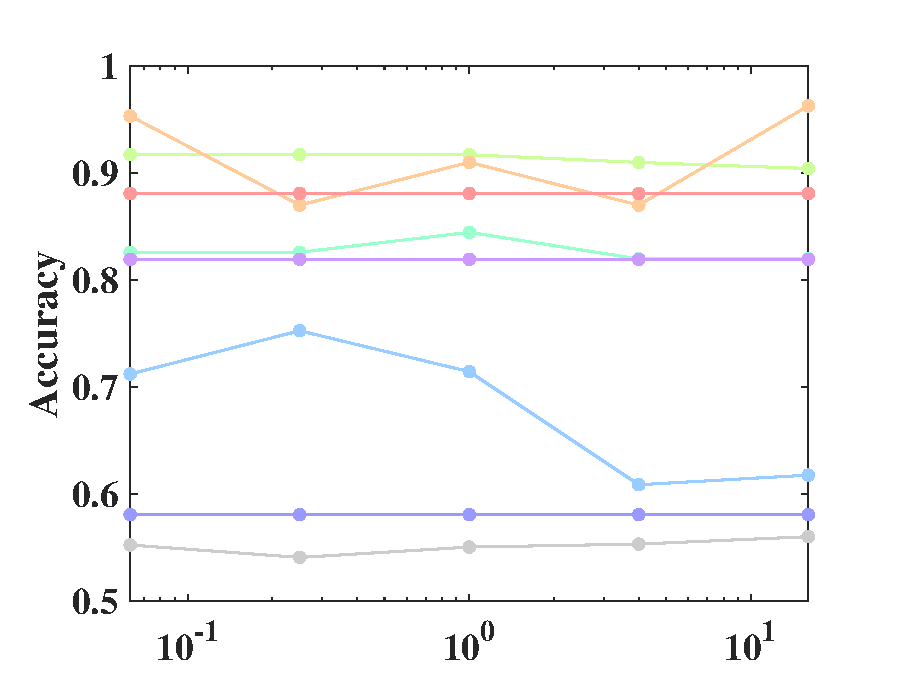
\includegraphics[width=0.3\textwidth]{C.eps}
        \label{C}
    }
   \hfill
    \subfigure[\text{$\lambda_1$}]{
        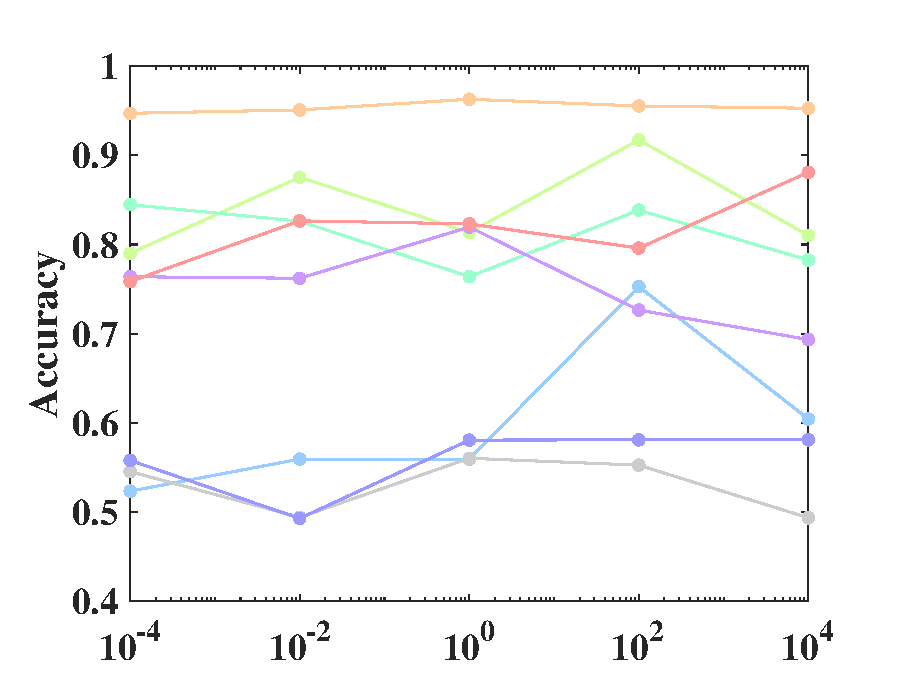
\includegraphics[width=0.3\textwidth]{lambda1.eps}
        \label{LPP}
    }
    \hfill
    \subfigure[\text{$\lambda_2$}]{
        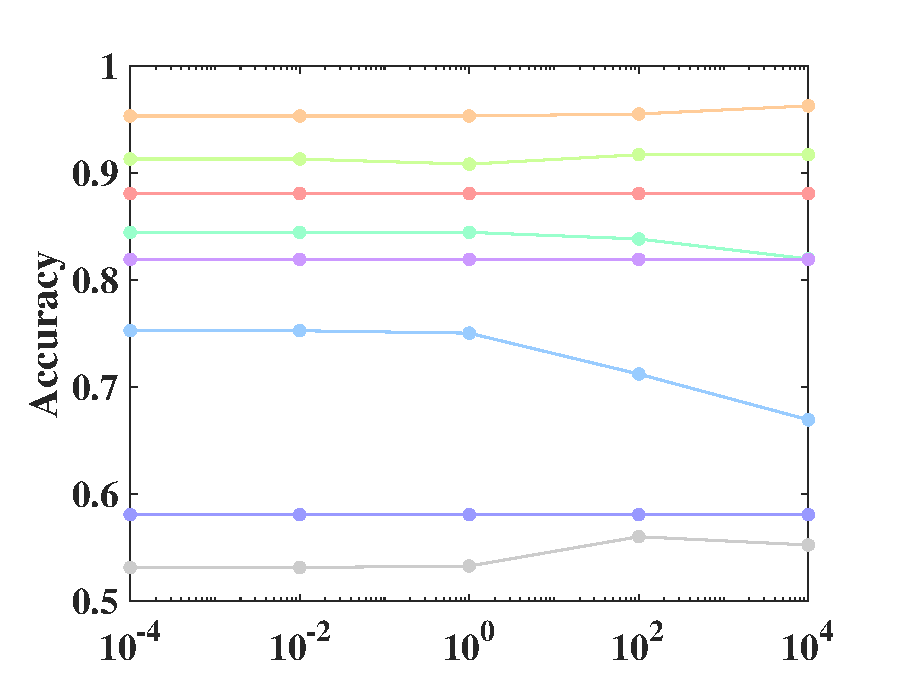
\includegraphics[width=0.3\textwidth]{lambda2.eps}
        \label{MDS}
    }
    
    %\vspace{1em} % Space between rows
    
    \subfigure[\text{$\lambda_3$}]{
        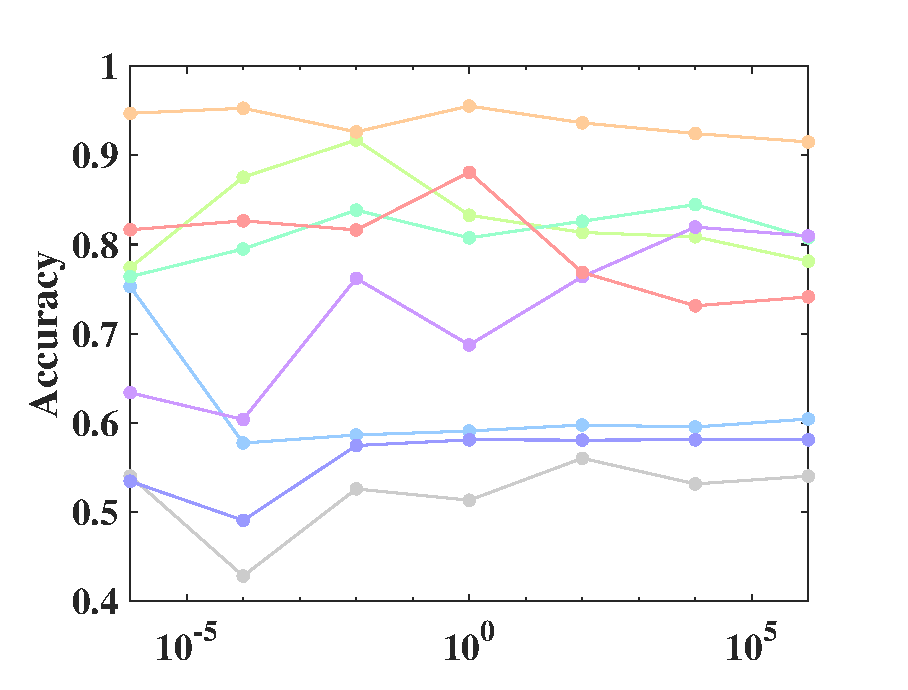
\includegraphics[width=0.3\textwidth]{lambda3.eps}
        \label{NCA}
    }
   \hfill
    \subfigure[\text{$\lambda_4$}]{ 
        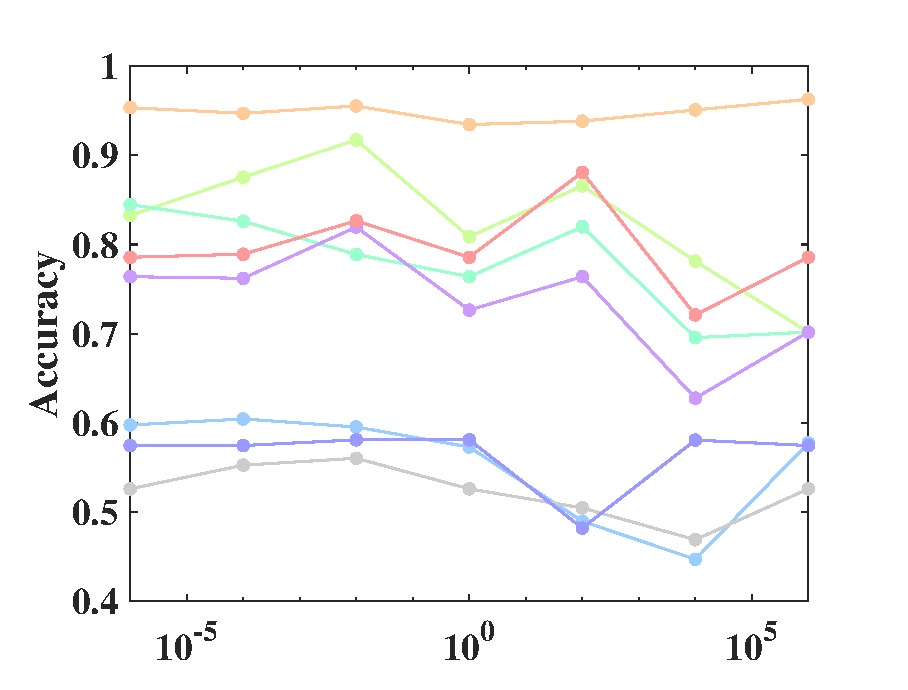
\includegraphics[width=0.3\textwidth]{lambda4.eps}
        \label{NPE}
    }
    \hfill
    \subfigure[\text{$\lambda_5$}]{ 
        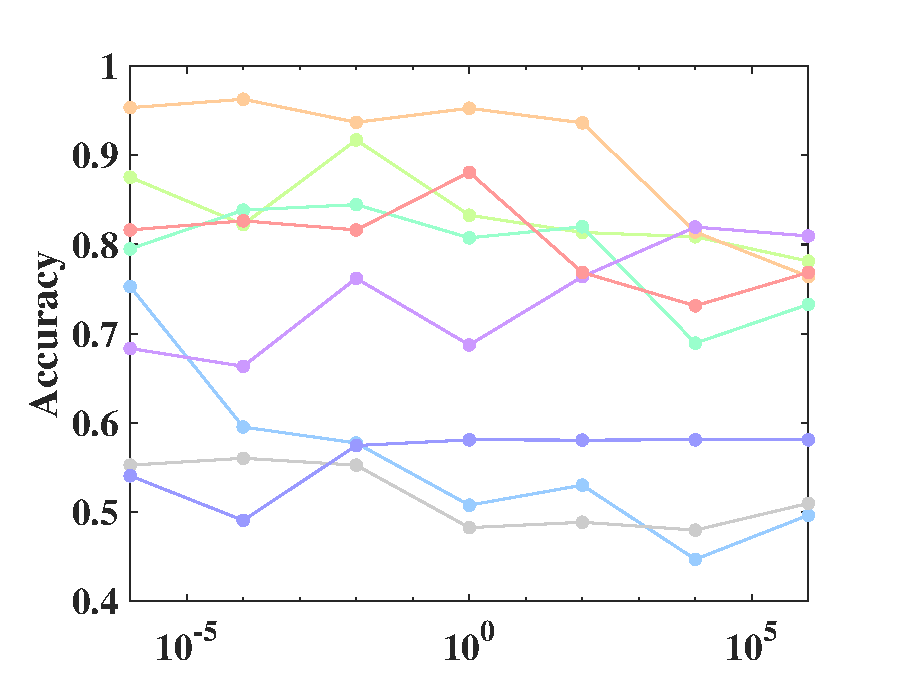
\includegraphics[width=0.3\textwidth]{lambda5.eps}
        \label{DRCA}
    }
    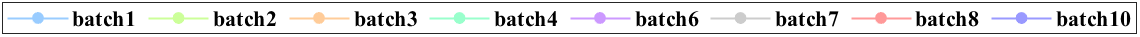
\includegraphics[width=0.8\textwidth]{1.png}
    
    \caption{Visualization of recognition accuracy of various parameters changing with batches.} 
    \label{six}
\end{figure*}

%实验动机
To further evaluate the stability of CDLDM, we conducted parameter sensitivity analysis under setting 1 using the UCSD dataset in this section.
CDLDM has six pivotal parameters: $C$, $\lambda_1$, $\lambda_2$, $\lambda_3$, $\lambda_4$, $\lambda_5$. 
% To determine the optimal values for the parameters mentioned, we employ a grid search method to evaluate the accuracy of each parameter at different values. 
We employ the grid search method to determine the optimal values for each parameter.
The specific experimental results are shown in Fig. \ref{six}.

%结果分析
Fig. \ref{six} depicts the accuracy variation trends of various parameters of the CDLDM algorithm on different batches.
% As shown in Fig. \ref{six}, we observe that the sensitivity curves of different parameters are different. 
% Due to the varying degrees of drift in different batches, the sensitivity of the same parameter varies under different batch conditions. 
% We can clearly see that C and $\lambda_2$ exhibit stable accuracy on the vast majority of batches. $\lambda_3$ is relatively stable when the value is large, while $\lambda_4$ is relatively stable when the value is small. 
We observe that $C$ and $\lambda_2$ consistently exhibit stable accuracy across the majority of batches. Meanwhile, $\lambda_3$ demonstrates relative stability when its value is large, whereas $\lambda_4$ maintains relative stability when its value is small.
$\lambda_1$ and $\lambda_5$ are relatively volatile, but they can still achieve optimal values across a wide range of values.
Based on these findings, we can efficiently identify the optimal value ranges for each parameter, which will facilitate our subsequent research.
% Based on this result, we can quickly determine the optimal range of values for each parameter, which is beneficial for our further research.



\subsection{Ablation study} \label{Abla}
%------------------------- Experiments 6 --------------------%
\begin{table*}[ht]
\centering
\setlength{\abovecaptionskip}{0pt}
\caption{UCSD dataset ablation classification accuracies under \textbf{Setting 1} (\%).}
\setlength{\tabcolsep}{3.2 mm}
\begin{tabular}{@{}ccccccccccccc@{}}
\toprule
 \multicolumn{10}{c}{Batch ID}  \\
\cmidrule(lr){2-10}
case & $5 \rightarrow 1$ & $5 \rightarrow 2$ & $5 \rightarrow 3$ & $5 \rightarrow 4$ & $9 \rightarrow 6$ & $9 \rightarrow 7$ & $9 \rightarrow 8$ & $9 \rightarrow 10$ & Average \\
\midrule
Scenario 1 & 41.80 & 55.23 & 39.85 & 63.35 & 22.70 & 17.96 & 70.07 & 18.28 & 44.42 \\
Scenario 2 & 56.18 & 67.77 & 53.91 & 83.23 & 30.96 & 35.18 & 58.50 & 32.39 & 55.10 \\
Scenario 3 & 52.58 & 81.27 & \bfseries{98.36} & 61.49 & 47.39 & 23.64 & 69.05 & 38.22 & 61.97 \\
Scenario 4 & 59.55 & 74.76 & 96.53 & 80.12 & 62.87 & 45.20 & 66.33 & 47.19 & 69.34 \\
Scenario 5 & 71.46 & 77.57 & 98.11 & 83.85 & 43.48 & 28.98 & 72.11 & 32.53 & 67.94 \\
Scenario 6 & 60.00 & 80.55 & 98.23 & 80.75 & 65.96 & 53.89 & 86.44 & 43.78 & 75.12 \\
Scenario 7 & 64.04 & 85.77 & 97.79 & 79.50 & 61.91 & 49.40 & 78.23 & 47.36 & 73.81 \\
CDLDM & \bfseries{75.28} & \bfseries{91.72} & 96.28 & \bfseries{84.47} & \bfseries{81.96} & \bfseries{56.05} & \bfseries{88.10} & \bfseries{58.11} & \bfseries{79.00} \\

\bottomrule
\end{tabular}
\label{ablation}
\end{table*}

%实验动机
% In order to investigate whether CDLDM significantly improves the performance of LDM when dealing with cross domain problems, we conduct a series of ablation experiments aimed at analyzing the impact of each component of CDLDM on overall performance. We conduct the following ablation experiments using the UCSD dataset under Setting 1.
In this section, we performed ablation experiments to illustrate that CDLDM substantially enhances the capability of LDM in cross-domain learning. A total of seven distinct scenarios require comparison:
% We conduct the above experiment using the UCSD dataset under setting 1.


\textbf{Scenario 1:} By setting all parameters $\lambda_5$, $\lambda_4$, and $\lambda_3$ to 0, we comprehensively examined the performance of CDLDM in handling cross domain problems when all key components fail. At this scenario, the CDLDM model degenerates into the traditional LDM model, which helps to understand the overall response capability of the model when all key factors fail.

\textbf{Scenario 2:} By setting $\lambda_4$ and $\lambda_3$ to 0 simultaneously, we investigat the performance of CDLDM when the marginal distribution differences and the scattering distribution differences are weakened.

\textbf{Scenario 3:} Simultaneously setting $\lambda_5$ and $\lambda_3$ to 0, we investigat the performance of CDLDM while reducing attention to the marginal distribution differences and the graph-based Laplacian regularization.

\textbf{Scenario 4:} By simultaneously setting $\lambda_5$ and $\lambda_4$ to 0, we delve into the performance of CDLDM when the scattering distribution differences and the graph-based Laplacian regularization are both weakened. This helps to reveal the overall adaptability of the model when the trade-off parameters in these two aspects fail simultaneously.

\textbf{Scenario 5:} By setting $\lambda_3$ to 0, we completely eliminate the focus on differences in marginal distribution. The target of this scenario is to assess the adaptability of CDLDM to cross domain problems while ignoring differences in marginal distribution, with a focus on examining the role of $\lambda_3$ in the model.

\textbf{Scenario 6:} Setting $\lambda_4$ to 0 eliminates the focus on scattering distribution differences. This setting aims to investigate in depth the performance of CDLDM in handling cross domain problems while reducing attention to scattering distribution differences, highlighting the unique contribution of $\lambda_4$ in overall performance.

\textbf{Scenario 7:} We set $\lambda_5$ to 0. This means that we have excluded the influence of the trade-off parameter $\lambda_5$ in graph based Laplacian regularization. Through this setting, we aim to evaluate the ability of CDLDM to handle cross domain problems while ignoring geometric information between samples, emphasizing the role of $\lambda_5$ in the model.
%结果分析

% The experimental results are shown in Table \ref{ablation}, which intuitively shows that deleting any component of the model will reduce the performance of the model. 
Table \ref{ablation} displays the results, revealing that omitting any component from the model results in diminished performance.
Specifically, the more components of the model are lost, the overall trend of the model decreases. And when all components are removed, that is, when CDLDM degenerates into LDM, the performance of the model is the lowest, with an average accuracy of only 44.42\%, which is 34.58\% lower than the proposed model CDLDM. Furthermore, we can observe that when the projection marginal distribution discrepancy component of the model is removed, the performance of the model will be greatly affected. From the results, we can see that, excluding scenario 7, almost all batches corresponding to the lowest performance are missing the component of projection marginal distribution discrepancy. Overall, whether a certain part or two parts are missing, it will have an impact on the performance of the model, and our proposed model does greatly improve the cross-domain processing ability of traditional LDM.


% \subsection{A Summary of Experimental Conclusions} \label{sum}
% \label{sum}
% ****


\section{Conclusion}\label{Conclu}
This paper proposes a novel cross-domain large margin distribution machine, aiming to solve the challenges faced by traditional support vector machines when processing sensor drift data. CDLDM aims to minimize the distribution discrepancy between source and target domains by simultaneously optimizing the projected maximum marginal distribution discrepancy, projected maximum distribution scattering discrepancy, and the manifold consistency under marginal distribution, thus achieving effective domain adaptation. In addition, CDLDM optimizes marginal distribution and achieves better generalization performance than SVM.
An extensive array of systematic experiments conducted across diverse E-nose datasets has consistently underscored the exceptional cross-domain learning capabilities demonstrated by the CDLDM algorithm. Although CDLDM demonstrates strong cross-domain learning capabilities, it necessitates the optimization of a large number of parameters. In the future, we will focus on developing effective parameter optimization methods to achieve optimal results more efficiently.
Overall, from the perspective of machine learning, we provide a new and efficient solution to the sensor drift problem. The proposed CDLDM is a domain adaptive classifier that has cross-domain capabilities and effectively solves the problem of distribution inconsistency caused by drift, providing a new perspective for exploring LDM theory.

%------------------------ Credit ------------------------
\printcredits


%------------------------ Declaration ------------------------
% \section*{Declaration of Competing Interest}
% The authors declare that they have no known competing financial interests or personal relationships that could have appeared to influence the work reported in this paper.


%------------------------ Acknowledgments ------------------------
% \section*{Acknowledgments}
% This work is supported by the National Natural Science Foundation of China (No. 62106205), the National Key Research and Development Program of China (No. 2021YFB3101500), the Youth project of science and technology research program of Chongqing Education Commission of China(No. KJQN202100207), and the Chongqing Municipal Training Program of Innovation and Entrepreneurship for Undergraduate (No. X202310635204).



%------------------------ Reference ------------------------

%\bibliographystyle{unsrtnat}
% \bibliography{ref}
%\begin{refcontext}[sorting = none]
% \hypersetup{
%   %colorlinks=true,
%   linkcolor=blue,
%   urlcolor=blue
% }

% \bibliographystyle{unsrtnat}
\bibliographystyle{model5-names} 
\bibliography{ref.bib}
%\end{refcontext}
\vfill

\end{document}
